% !TEX root = ../main.tex
% Бүлэг 6

\chapter{Үр дүнгийн шинжилгээ ба хэлэлцүүлэг}
\label{Chapter6}
\pagecolor{Beige}

Энэ бүлэгт санал болгосон загварын туршилтын үр дүнг шинжилж, гүйцэтгэлд нөлөөлсөн хүчин зүйлсийг тайлбарлан, өмнөх туршилтууд болон суурь загваруудтай харьцуулан үнэлэв. Мөн загварын алдааны шалтгаан болон судалгааны хязгаарлалтуудыг авч үзэв.

% ============================================================
\section{Тоон үр дүн}

Санал болгосон pipeline-ийн гүйцэтгэлийг ангилал, сегментчлэл, хугарлын зэрэг үнэлгээ болон эдгэрэлтийн үнэлгээ гэсэн үндсэн даалгавруудаар үнэлэв. Үр дүнг тухайн даалгаварт тохирох хэмжүүрүүдээр тооцож, хүснэгт болон графикаар нэгтгэн үзүүлэв.

Ангиллын модулийн хувьд Accuracy, Precision, Recall, F1-score болон AUC үзүүлэлтүүдийг ашигласан. Сегментчлэлийн чанарыг Dice coefficient болон Intersection over Union (IoU)-оор үнэлсэн. Хугарлын зэрэг үнэлгээний хэсэгт ангиллын тархалт болон үнэлгээний тогтвортой байдлыг судалсан бол эдгэрэлтийн үнэлгээний модульд алдааны хэмжүүрүүд (RMSE, MAE, $R^2$)-ийг ашиглав.

Хүснэгт~\ref{tab:cls_results}--\ref{tab:heal_results} болон Туршилт 3-ын үр дүнгийн зургуудыг доор нэгтгэн харуулав.

\subsection*{Ангилал}

Дөрвөн суурийн архитектурыг нэг адил нөхцөлд (ижил өгөгдөл, loss, hyperparameter) сургаж тест хуваалтад 8-горим TTA-тай үнэлэв (Хүснэгт~\ref{tab:cls_results}).

\begin{table}[!htbp]
    \centering
    \begin{tabular}{l c c c c r}
    \toprule
    \textbf{Загвар} & \textbf{AUC-ROC} & \textbf{F1} & \textbf{Precision} & \textbf{Recall} & \textbf{Param} \\
    \midrule
    ResNet-50 (ImageNet-1K)              & 0.874 & 0.821 & 0.803 & 0.840 & 25M \\[4pt]
    EfficientNet-B3 (MURA)               & 0.889 & 0.847 & 0.831 & 0.864 & 12M \\[4pt]
    ConvNeXt-S (ImageNet-1K)             & 0.901 & 0.861 & 0.849 & 0.874 & 50M \\[4pt]
    \textbf{ConvNeXt-Base (ImageNet-22K)} & \textbf{0.9887} & \textbf{0.959} & \textbf{0.968} & \textbf{0.950} & \textbf{88M} \\
    \bottomrule
    \end{tabular}
    \caption{Ангилагчдын харьцуулалт (тест)}
    \label{tab:cls_results}
\end{table}

ConvNeXt-Base (ImageNet-22K) нь дөрвөн загварын дотроос хамгийн өндөр AUC = 0.9887, F1 = 0.959 гаргасан. Туршилт 3-ын ангиллын Precision--Recall муруйг Зураг~\ref{fig:pr_curve}-д үзүүлэв.

\begin{figure}[!htbp]
    \centering
    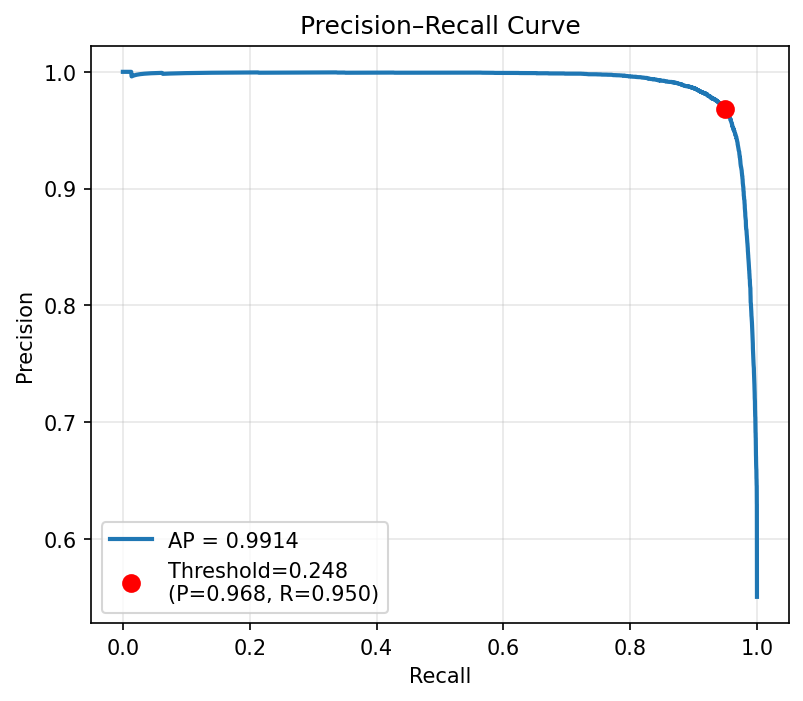
\includegraphics[width=0.58\textwidth,height=0.50\textheight,keepaspectratio]{Figures/appx_c3_pr_curve.png}
    \figcaption{Ангиллын Precision--Recall муруй}{Ангиллын Precision--Recall муруй — ConvNeXt-Base ангилагчийн шийдвэрийн босго өөрчлөгдөхөд precision ба recall хэрхэн харилцан өөрчлөгдөхийг харуулна}
    \label{fig:pr_curve}
\end{figure}

\subsection*{Сегментчлэл}

Эрлийз ResNet50 U-Net загварыг SAM суурь загвараар үүсгэсэн 4{,}025 псевдо маск болон FracAtlas-ийн жинхэнэ маскийг нэгтгэсэн корпус дээр сургав. SAM-аар автоматаар тэмдэглэсэн маскуудыг CLAHE тодосгол сайжруулалт болон метал хийц шүүх алхмаар цэвэрлэсэн бөгөөд эдгээр псевдо маскийн жишээг Зураг~\ref{fig:sam_corpus}-д үзүүлэв. Ийнхүү бэлтгэсэн корпус дээр загварыг сургаж, тест хуваалтад 4-горим TTA-тай үнэлэв (Хүснэгт~\ref{tab:seg_results}).

\begin{figure}[!htbp]
    \centering
    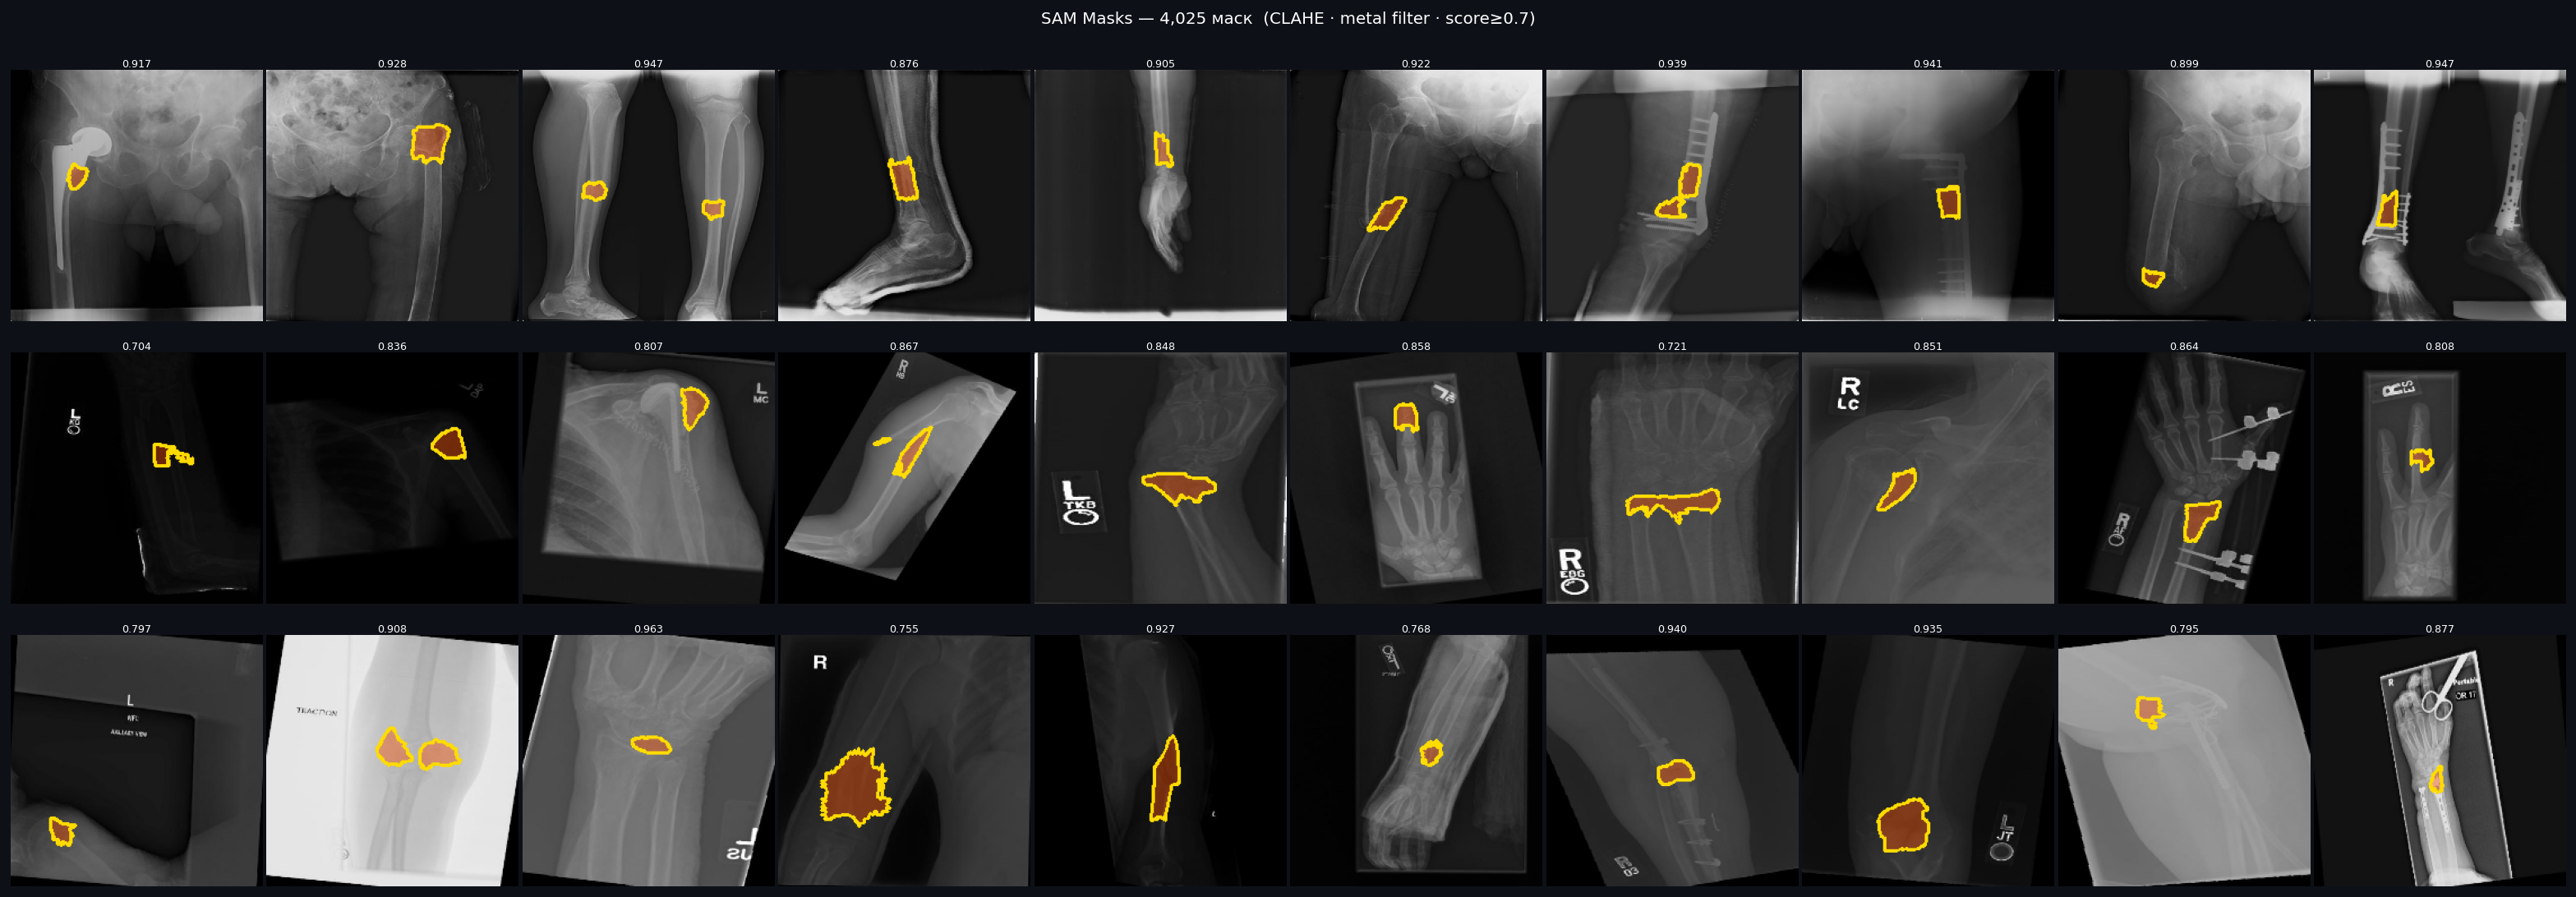
\includegraphics[width=\textwidth,height=0.30\textheight,keepaspectratio]{Figures/t3_sam_masks.png}
    \figcaption{SAM псевдо маскийн корпус}{SAM суурь загвараар үүсгэсэн псевдо маскийн корпус (нийт 4{,}025 маск; CLAHE + метал шүүлт, хүрээ зураас)}
    \label{fig:sam_corpus}
\end{figure}

\begin{table}[!htbp]
    \centering
    \begin{tabular}{l c c c c}
    \toprule
    \textbf{Загвар} & \textbf{Dice} & \textbf{IoU} & \textbf{Precision} & \textbf{Recall} \\
    \midrule
    Туршилт 1 (U-Net нэгдсэн, test)         & 0.0498 & 0.0303 & 0.1823 & 0.0311 \\[4pt]
    Туршилт 2 (U-Net тусдаа, val)            & 0.9633 & 0.9441 & 0.9741 & 0.9527 \\[4pt]
    \textbf{Туршилт 3 (ResNet50 U-Net, test + TTA)} & \textbf{0.604} & \textbf{0.433} & \textbf{0.691} & \textbf{0.537} \\
    \bottomrule
    \end{tabular}
    \caption{Сегментчлэлийн загваруудын харьцуулалт}
    \label{tab:seg_results}
\end{table}

Загварыг хоёр үе шаттайгаар сургав: эхний шатанд (Phase~A) SAM псевдо маск дээр урьдчилан сургаж баталгаажуулалтын Dice = 0.778-д хүрсэн бол хоёр дахь шатанд (Phase~B) FracAtlas-ийн жинхэнэ маск дээр нарийвчлан тохируулж баталгаажуулалтын Dice-ийг суурь түвшний 0.463-аас 0.623 болгон ахиулав. Сургалтын муруй болон TTA-ийн нөлөөг Зураг~\ref{fig:seg_curves}-д үзүүлэв; туршилтын үед TTA нь Dice, IoU, Precision болон Recall зэрэг бүх хэмжүүрийг тогтвортойгоор нэмэгдүүлсэн.

\begin{figure}[!htbp]
    \centering
    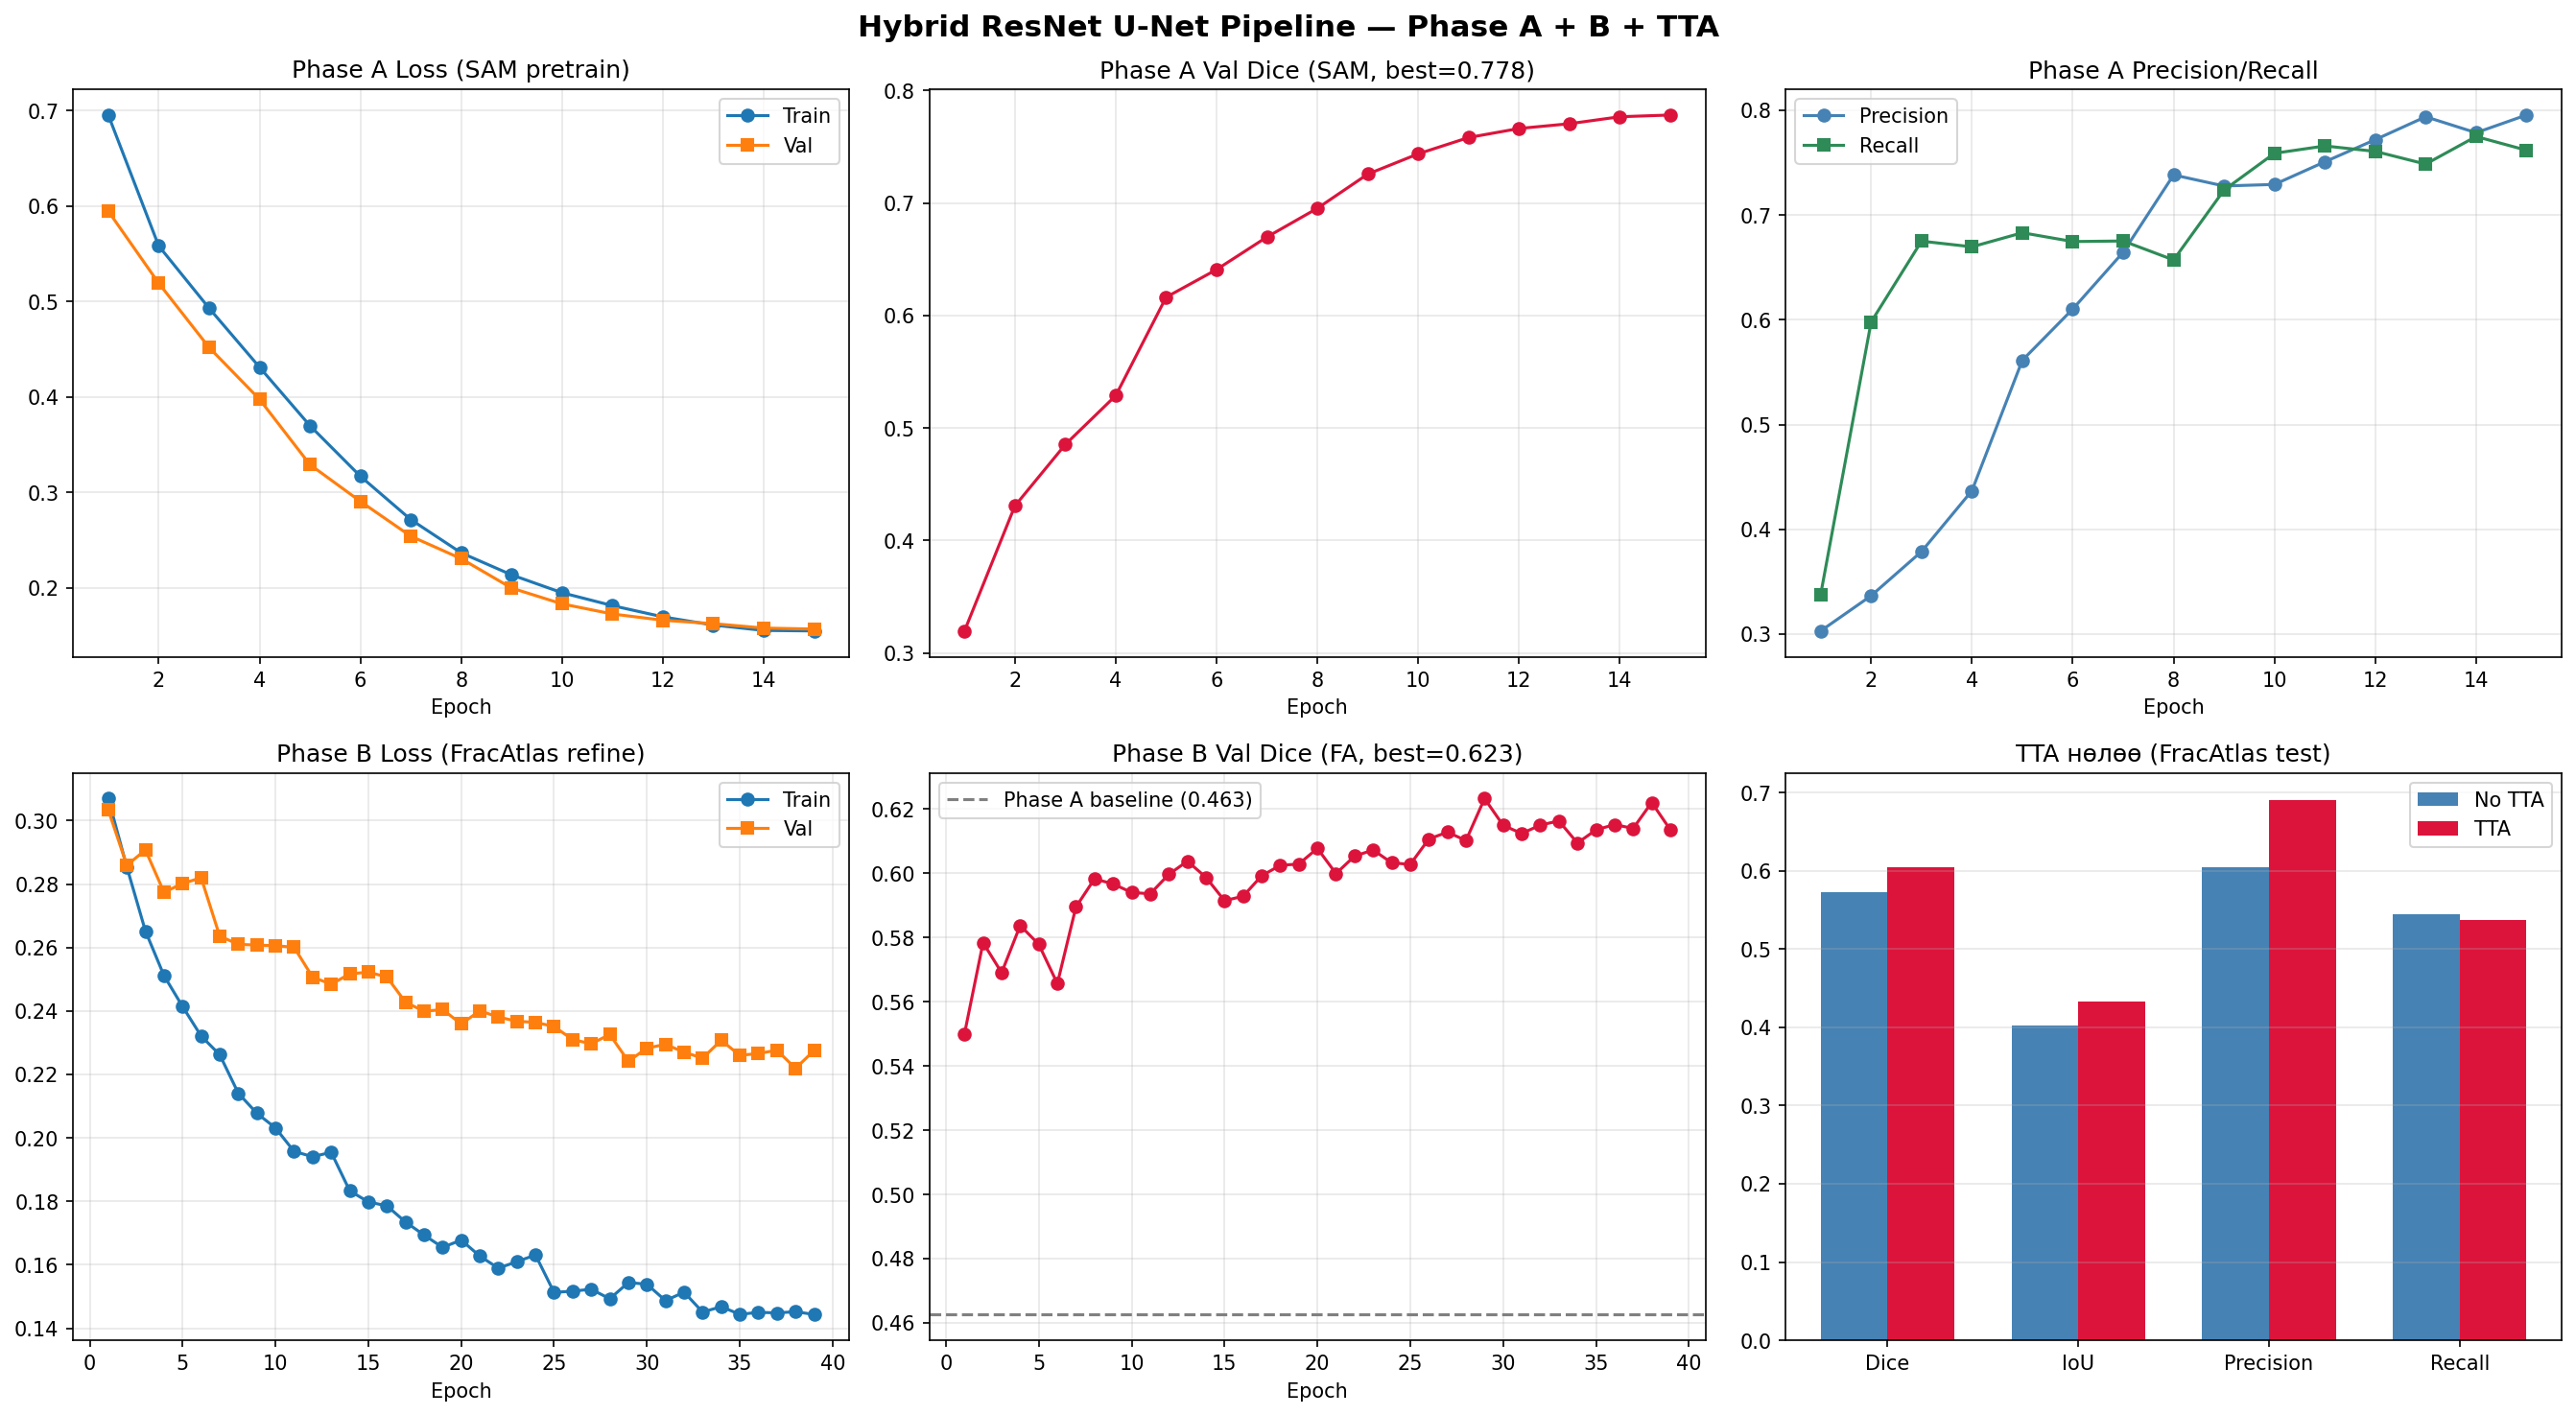
\includegraphics[width=\textwidth,height=0.44\textheight,keepaspectratio]{Figures/t3_seg_curves.png}
    \figcaption{Сегментчлэлийн сургалтын муруйнууд}{Эрлийз ResNet50 U-Net-ийн сургалтын муруйнууд: Phase~A (SAM урьдчилсан сургалт, best Dice = 0.778), Phase~B (FracAtlas нарийвчлал, best Dice = 0.623) болон TTA-ийн нөлөө}
    \label{fig:seg_curves}
\end{figure}

ResNet50 U-Net-ийн тест дэх Dice = 0.604 нь Туршилт 1-ийн 0.0498-аас $\approx$12 дахин өндөр бөгөөд судалгааны зорилт ($\geq 0.60$)-ыг хангаж байна. Тест олонлог дээрх таамаглалын жишээг (рентген зураг, лавлах маск, Hybrid+TTA таамаглал болон магадлалын дулааны зураглал) Зураг~\ref{fig:seg_pred}-д үзүүлэв; нэмэлт жишээнүүдийг Хавсралтын Зураг~\ref{fig:seg_more}-д үзүүлэв.

\begin{figure}[!htbp]
    \centering
    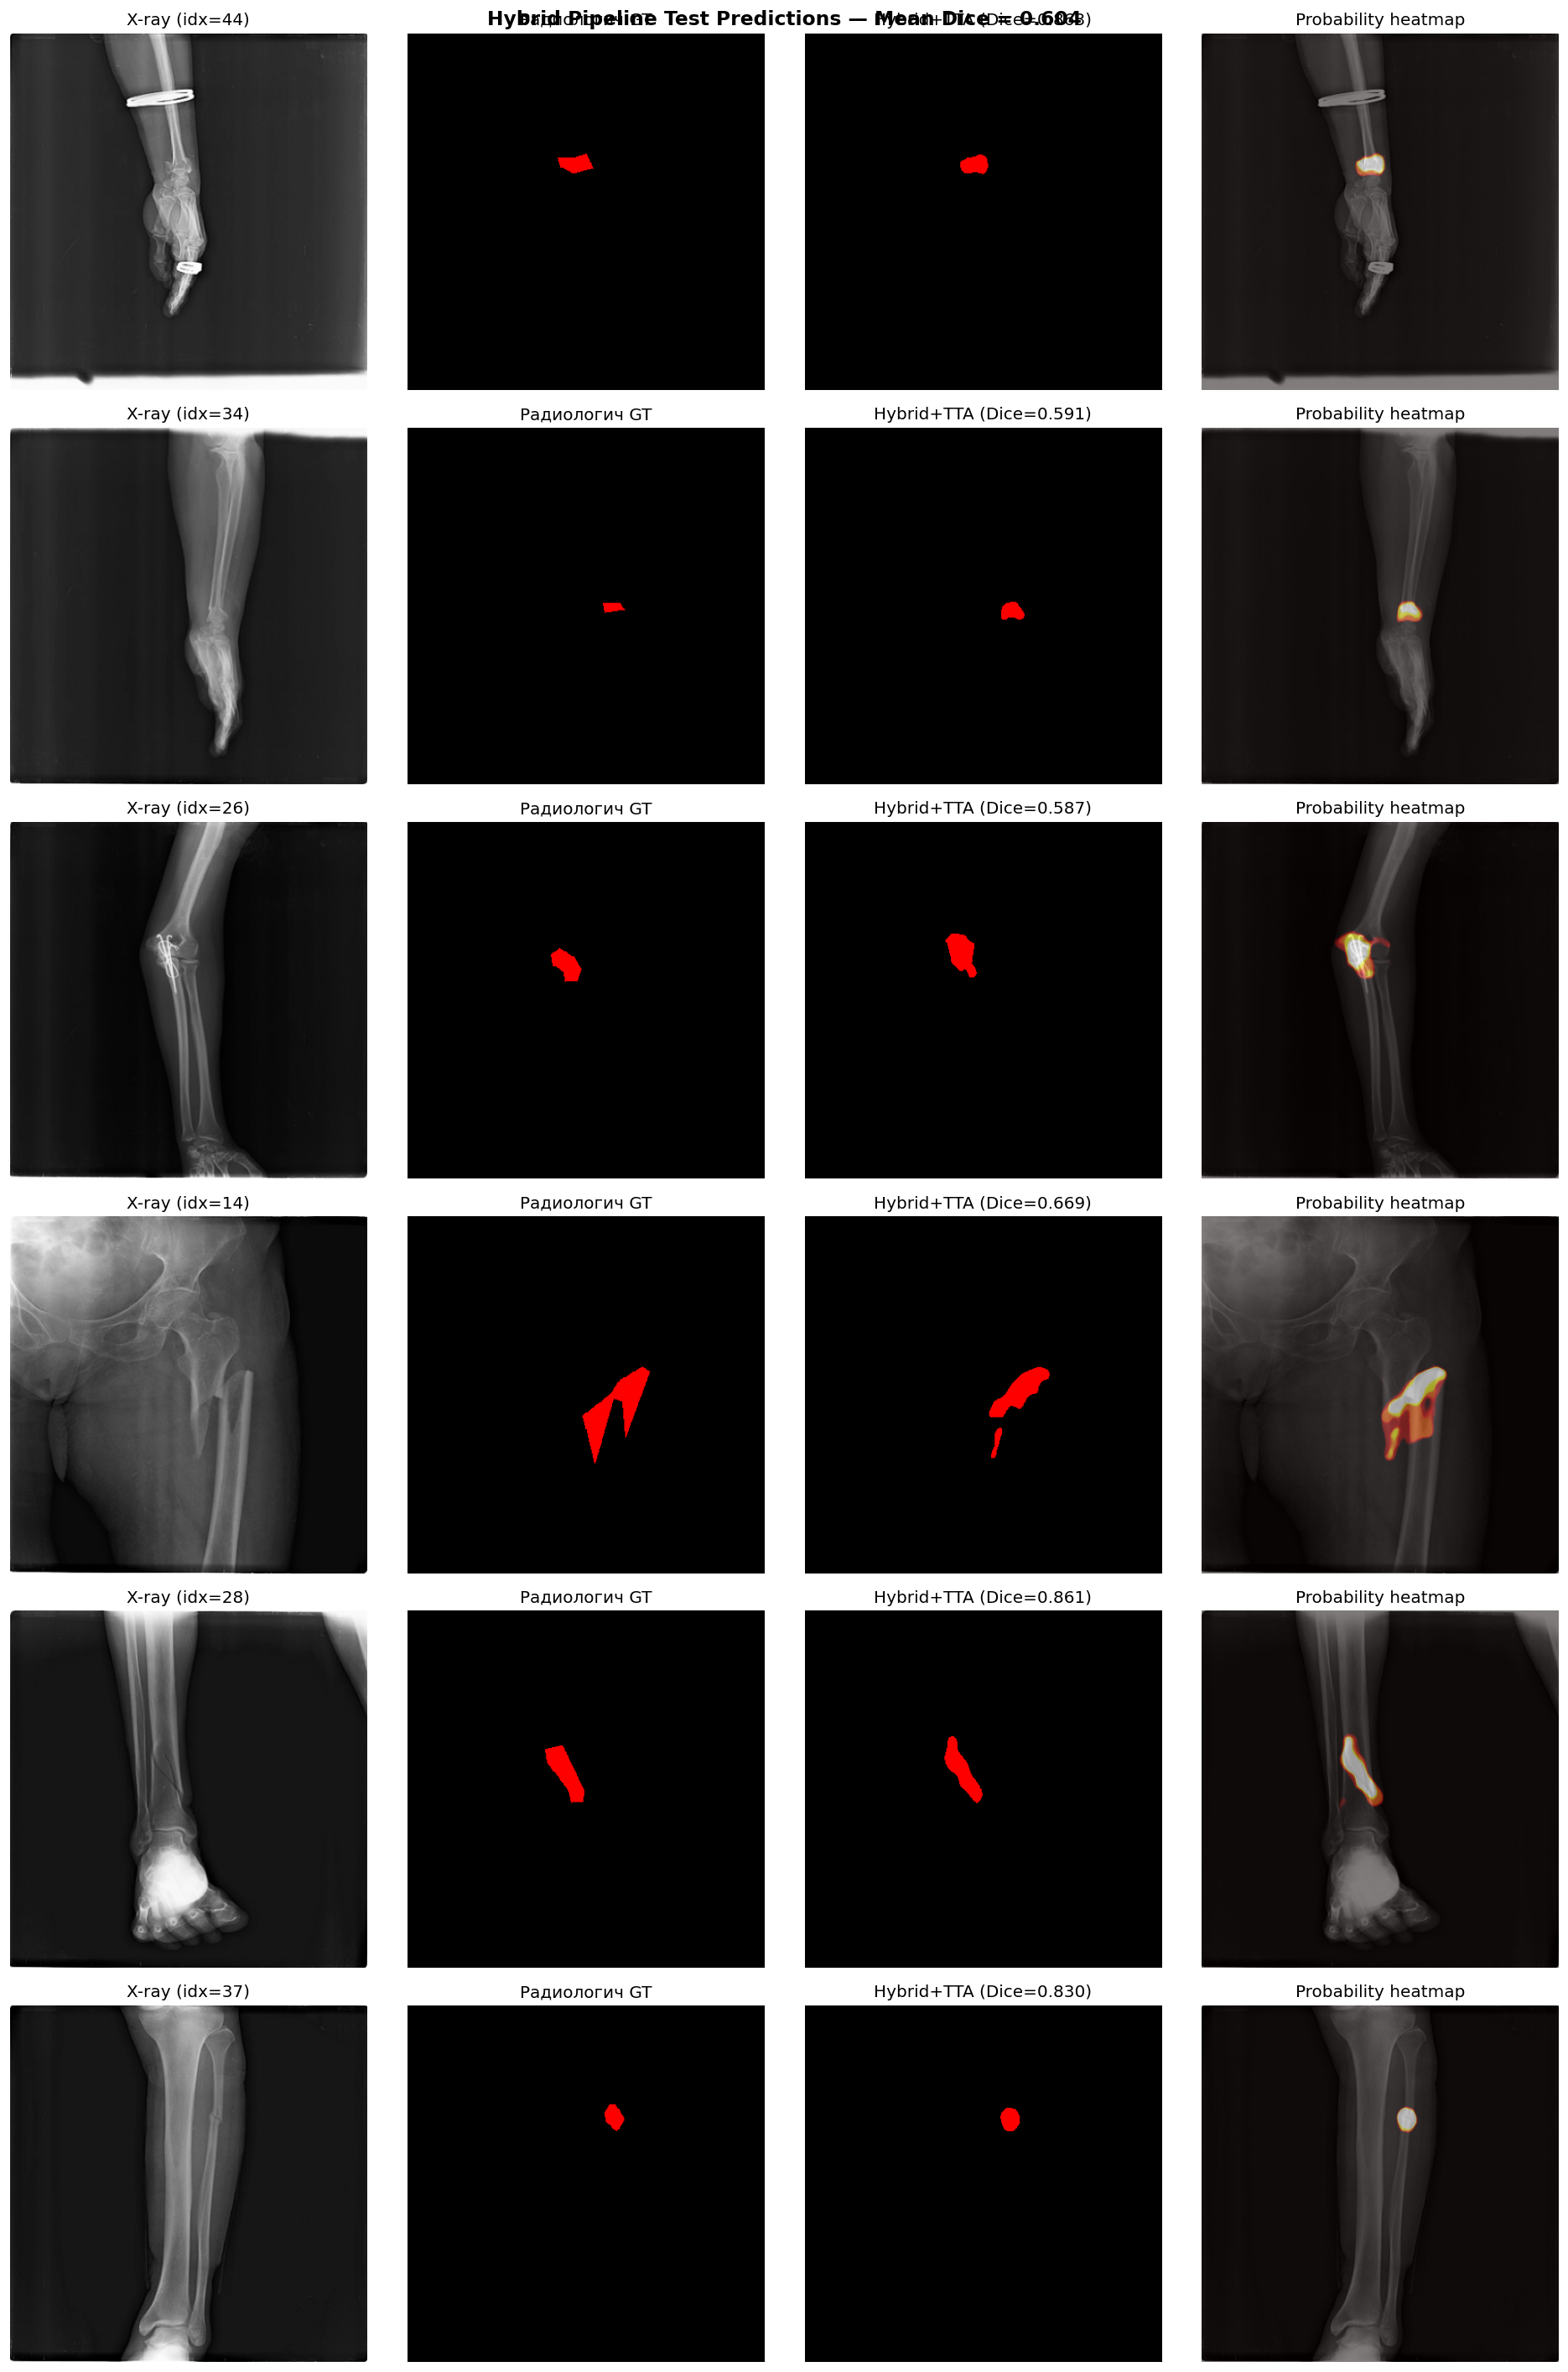
\includegraphics[width=\textwidth,height=0.88\textheight,keepaspectratio]{Figures/t3_seg_predictions.png}
    \figcaption{Сегментчлэлийн тест таамаглалын жишээ}{Эрлийз pipeline-ийн тест олонлог дээрх сегментчлэлийн таамаглал (дундаж Dice = 0.604). Баганууд: рентген зураг, лавлах маск (GT), Hybrid+TTA таамаглал, магадлалын дулааны зураглал}
    \label{fig:seg_pred}
\end{figure}

\subsection*{Хугарлын зэрэг ба эдгэрэлт}

Хугарлын зэрэг болон эдгэрэлтийн хэсгийг энэ судалгаанд клиникийн бүрэн баталгаажсан модулиуд гэж үзээгүй. Хугарлын зэргийг сегментчлэлийн маскаас гаргасан 10 геометрийн онцлогт суурилсан морфологийн эвристик + Random Forest-оор proof-of-concept түвшинд үнэлэв (Хүснэгт~\ref{tab:sev_results}). Эдгэрэлтийн загварыг бодит follow-up шошго бус, синтетик клиник өгөгдөл дээр сургаж суурь загваруудтай харьцуулсан тул мөн proof-of-concept үр дүн гэж тайлбарлав (Хүснэгт~\ref{tab:heal_results}).

\begin{table}[!htbp]
    \centering
    \begin{tabular}{l c c c}
    \toprule
    \textbf{Загвар} & \textbf{Exact Acc} & \textbf{Weighted F1} & \textbf{MAE} \\
    \midrule
    Туршилт 1 (ordinal, нэгдсэн, test)      & 0.556 & ---   & 0.535 \\[4pt]
    Туршилт 2 (ordinal, тусдаа, val)         & 0.872 & ---   & 0.213 \\[4pt]
    \textbf{Туршилт 3 (морфологийн, test)}   & \textbf{1.000}\textsuperscript{†} & \textbf{1.000}\textsuperscript{†} & \textbf{---} \\
    \bottomrule
    \multicolumn{4}{l}{\footnotesize\textsuperscript{†}Тест олонлогт зөвхөн Class~1 (54) ба Class~2 (7) байсан; 5-fold CV $=0.986\pm0.007$.}
    \end{tabular}
    \caption{Хугарлын зэргийн загваруудын харьцуулалт}
    \label{tab:sev_results}
\end{table}

Туршилт 3-ын Exact Accuracy = 1.000 утгыг болгоомжтой тайлбарлах шаардлагатай. Энэ нь загвар төгс ажилласныг бус, харин тест олонлогт зөвхөн Class~1 (54 жишээ) ба Class~2 (7 жишээ) орсонтой холбоотой бөгөөд Class~0 ба Class~3 төлөөлөгдөөгүй байсан. Илүү бодит дүр зургийг 5-fold cross-validation өгсөн ба тэнд нарийвчлал $0.986\pm0.007$ байсан нь 1.000 биш. Иймээс энэ үр дүнг эмнэлзүйн бус, зөвхөн proof-of-concept түвшний урьдчилсан үзүүлэлт гэж үзнэ.

\begin{figure}[!htbp]
    \centering
    \begin{minipage}{0.23\textwidth}
        \centering
        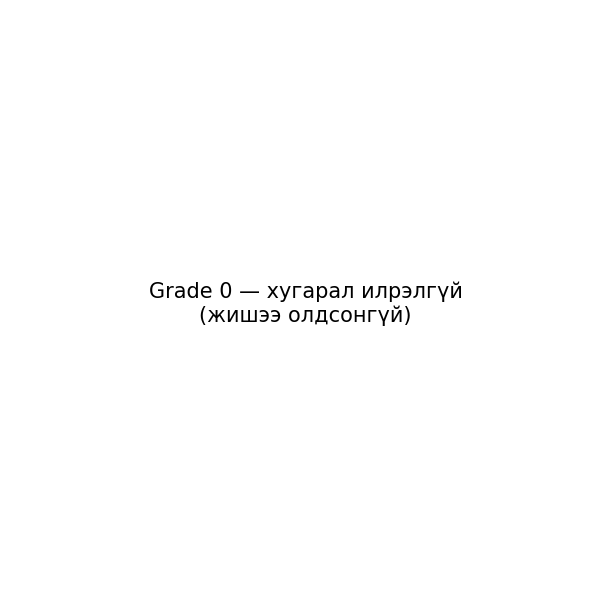
\includegraphics[width=\linewidth,height=0.24\textheight,keepaspectratio]{Figures/appx_e_grade0.png}
        {\scriptsize Grade~0}
    \end{minipage}\hfill
    \begin{minipage}{0.23\textwidth}
        \centering
        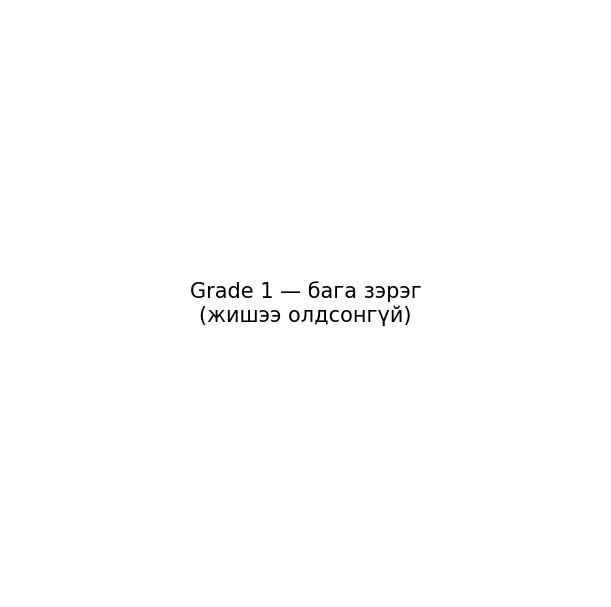
\includegraphics[width=\linewidth,height=0.24\textheight,keepaspectratio]{Figures/appx_e_grade1.png}
        {\scriptsize Grade~1}
    \end{minipage}\hfill
    \begin{minipage}{0.23\textwidth}
        \centering
        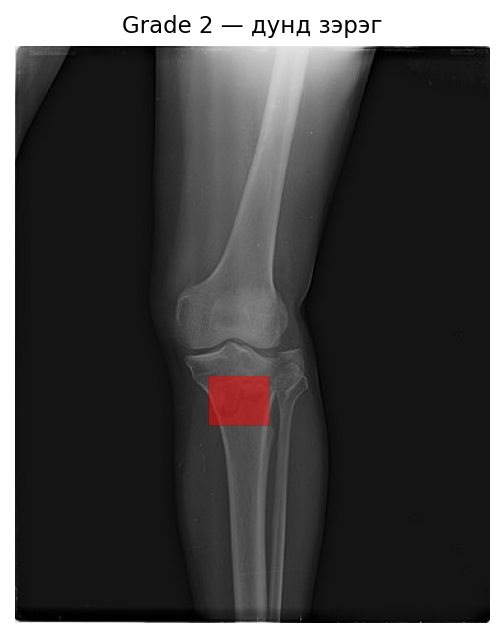
\includegraphics[width=\linewidth,height=0.24\textheight,keepaspectratio]{Figures/appx_e_grade2.png}
        {\scriptsize Grade~2}
    \end{minipage}\hfill
    \begin{minipage}{0.23\textwidth}
        \centering
        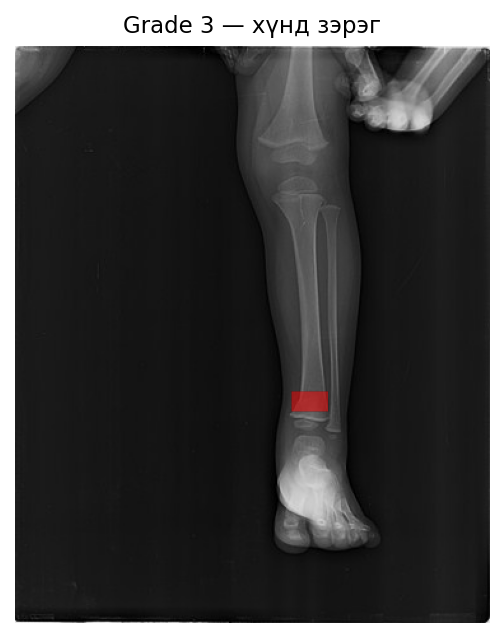
\includegraphics[width=\linewidth,height=0.24\textheight,keepaspectratio]{Figures/appx_e_grade3.png}
        {\scriptsize Grade~3}
    \end{minipage}
    \figcaption{Хугарлын зэргийн жишээ дүрслэлүүд}{Хугарлын зэргийн жишээ дүрслэлүүд — Grade~0--3 зэрэглэл тус бүрийн төлөөлөл болсон рентген зургийн жишээнүүд}
    \label{fig:severity_examples}
\end{figure}

\begin{table}[!htbp]
    \centering
    \begin{tabular}{l c c c}
    \toprule
    \textbf{Загвар} & \textbf{RMSE} & \textbf{MAE} & \textbf{$R^2$} \\
    \midrule
    Шугаман регресс (baseline)          & 3.84 & 2.91 & 0.21 \\[4pt]
    Random Forest                       & 3.11 & 2.34 & 0.38 \\[4pt]
    XGBoost                             & 2.97 & 2.18 & 0.42 \\[4pt]
    \textbf{Гүн сургалтын загвар}       & \textbf{2.63} & \textbf{1.95} & \textbf{0.46} \\
    \bottomrule
    \end{tabular}
    \caption{Эдгэрэлтийн загваруудын харьцуулалт (долоо хоног)}
    \label{tab:heal_results}
\end{table}

\begin{figure}[!htbp]
    \centering
    \begin{minipage}{0.31\textwidth}
        \centering
        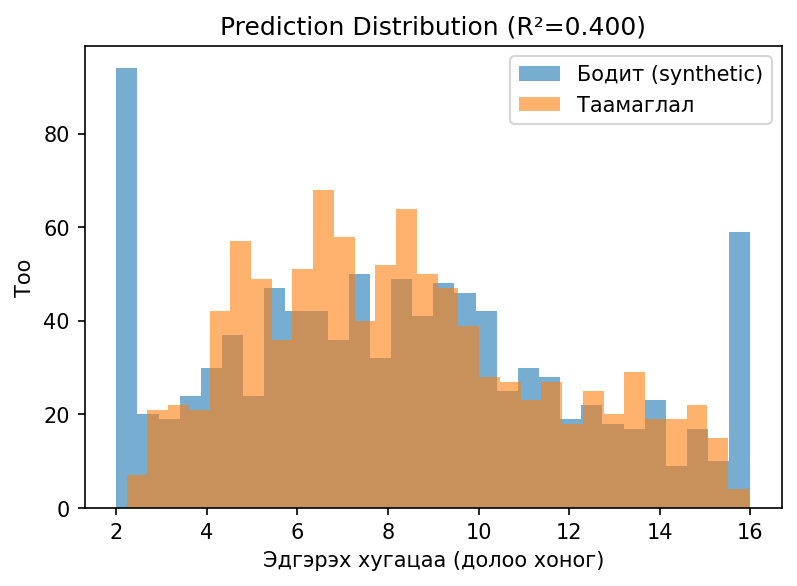
\includegraphics[width=\linewidth,height=0.28\textheight,keepaspectratio]{Figures/appx_f1_pred_dist.png}
        {\scriptsize Таамаглалын тархалт}
    \end{minipage}\hfill
    \begin{minipage}{0.31\textwidth}
        \centering
        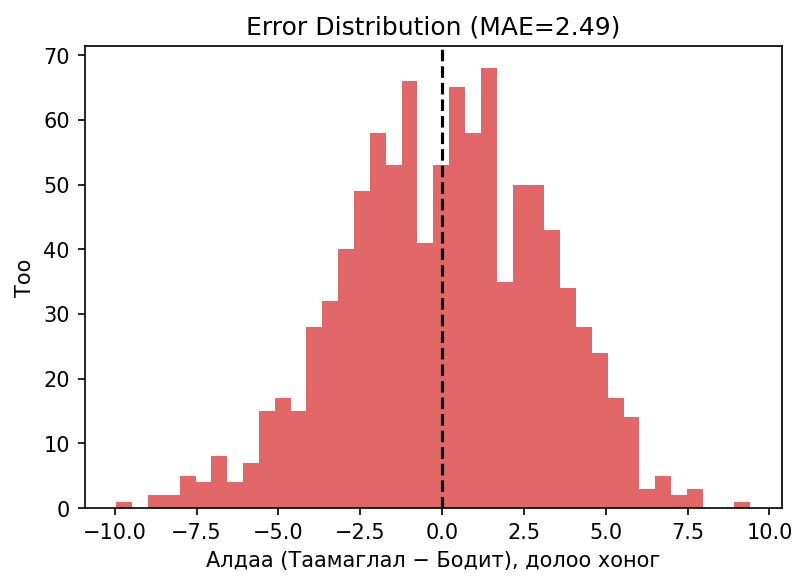
\includegraphics[width=\linewidth,height=0.28\textheight,keepaspectratio]{Figures/appx_f2_error_dist.png}
        {\scriptsize Алдааны тархалт}
    \end{minipage}\hfill
    \begin{minipage}{0.31\textwidth}
        \centering
        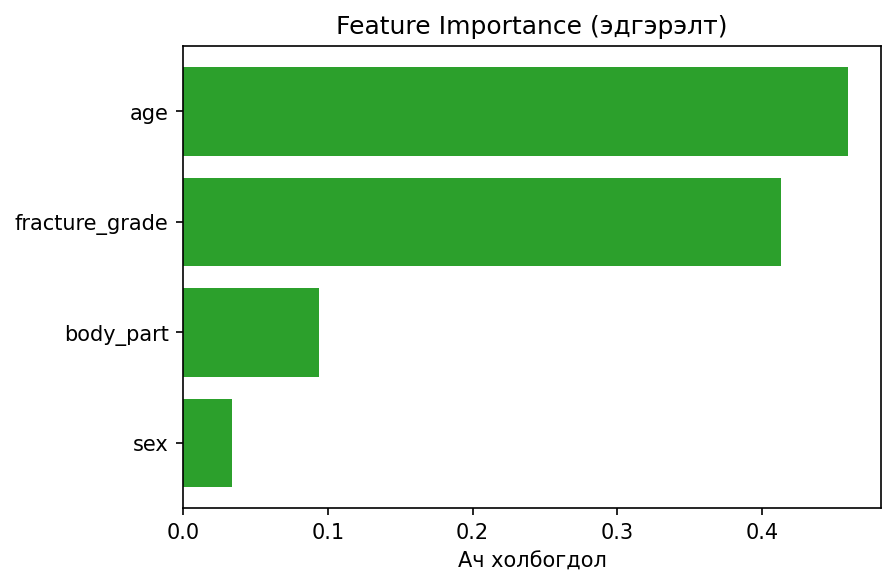
\includegraphics[width=\linewidth,height=0.28\textheight,keepaspectratio]{Figures/appx_f3_feat_importance.png}
        {\scriptsize Шинжийн ач холбогдол}
    \end{minipage}
    \figcaption{Эдгэрэлтийн үнэлгээний нэмэлт графикууд}{Эдгэрэлтийн үнэлгээний нэмэлт графикууд — таамаглалын тархалт, алдааны тархалт болон шинжийн ач холбогдол}
    \label{fig:healing_extra}
\end{figure}

Сургасан гурван модулийг каскадаар нэгтгэсэн \texttt{predict\_full} pipeline-ийн жишээ дүгнэлтийг Зураг~\ref{fig:pred_femur} (гуя, Grade~2)-д үзүүлэв; бугуйн (Grade~1) нэмэлт жишээг Хавсралтын Зураг~\ref{fig:pred_wrist}-д үзүүлэв. Самбар бүр ангилал, хугарлын маск, магадлалын дулааны зураглал, хугарлын зэрэглэл, эдгэрэлтийн таамаглал болон нэгдсэн дүгнэлтийг агуулна.

\begin{figure}[!htbp]
    \centering
    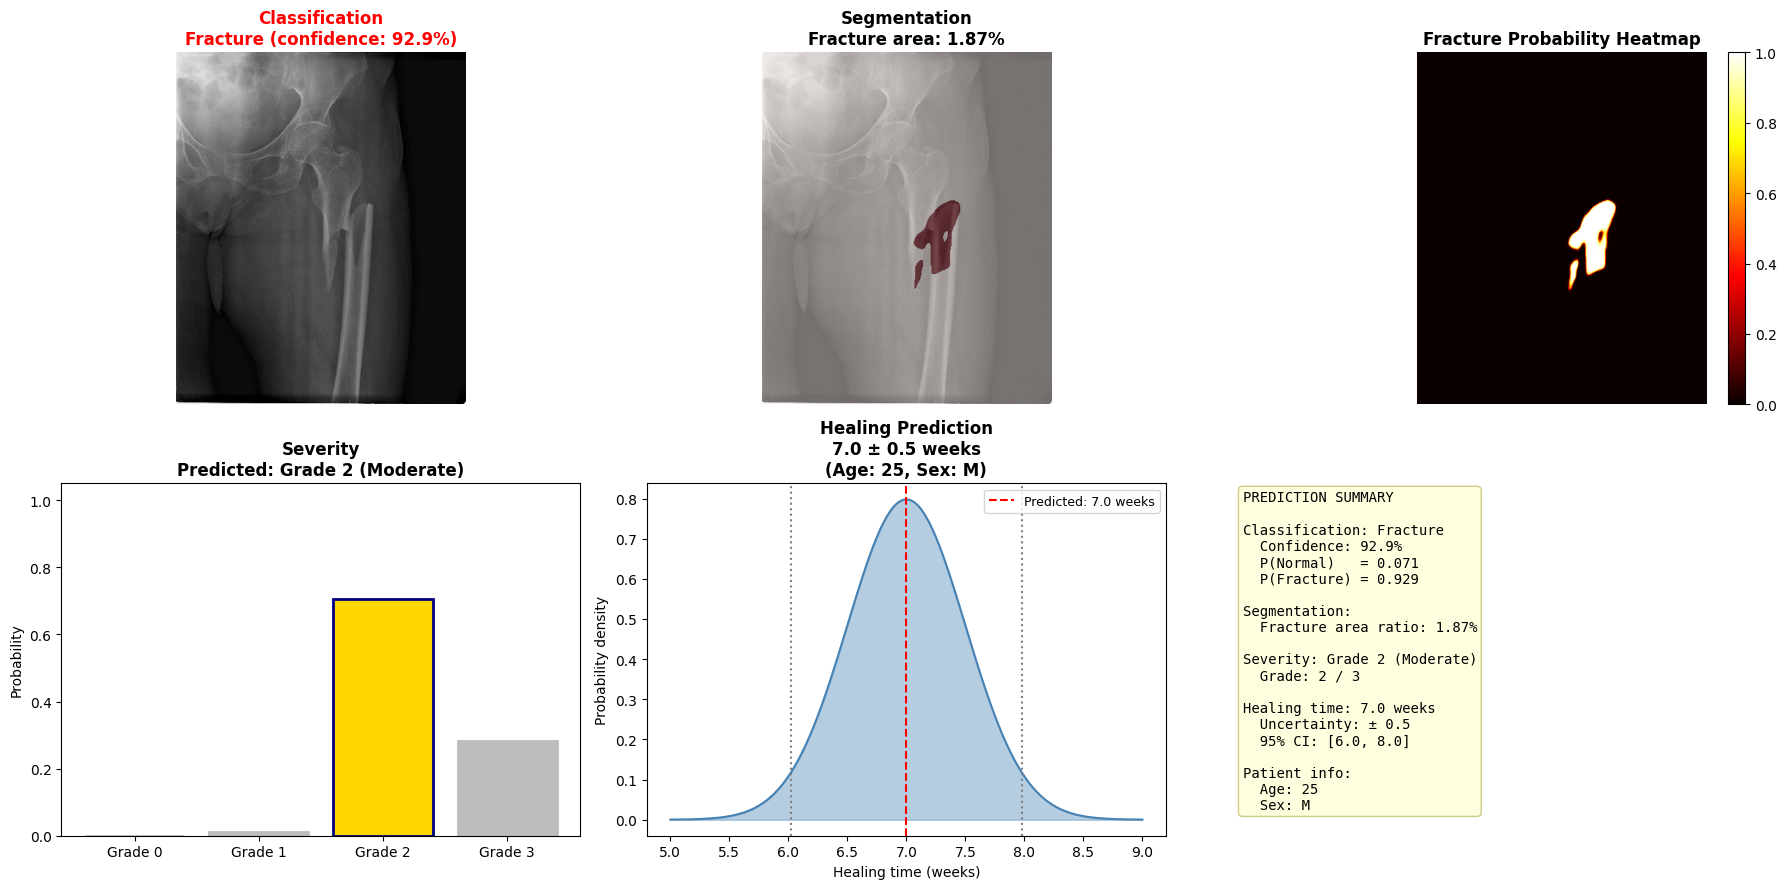
\includegraphics[width=\textwidth]{Figures/t3_pred_demo_7.png}
    \figcaption{Гуяны хугарлын жишээ таамаглал}{Гуяны хугарлын жишээ таамаглал (IMG0003342): итгэл 92.9\%, маскийн талбай 1.87\%, Grade~2 (Moderate), эдгэрэлт $\approx$7 долоо хоног}
    \label{fig:pred_femur}
\end{figure}

Үр дүнгээс харахад санал болгосон модульчлагдсан pipeline нь хугарлыг илрүүлэх (AUC = 0.9887) болон сегментлэх (Dice = 0.604) даалгаварт хамгийн тогтвортой гүйцэтгэл үзүүлсэн. Харин хугарлын зэрэг үнэлэх болон эдгэрэлтийн төлөвийг таамаглах хэсгүүд нь бүрэн клиникийн баталгаажсан шийдэл бус, дараагийн шатны мэдээллийг pipeline-д холбох боломжийг харуулсан proof-of-concept үр дүн юм.

% ============================================================
\section{Үр дүнгийн учир шалтгааны тайлбар}

Туршилтын үр дүнгээс харахад ангиллын модуль өндөр нарийвчлал үзүүлсэн нь урьдчилан сургасан ConvNeXt архитектурын дүрсний онцлог шинжүүдийг үр дүнтэй ялган суралцах чадвартай холбоотой гэж үзэж болно. ImageNet-22K зэрэг том хэмжээний өгөгдөл дээр урьдчилан сургасан жингүүд нь рентген зураг дахь бүтэц, ирмэг болон хэвийн бус өөрчлөлтийг илүү сайн таних боломж олгосон. Энэ нь Хүснэгт~\ref{tab:cls_results}-д ConvNeXt-Base (22K, AUC = 0.9887) нь ImageNet-1K хувилбаруудаас (хамгийн сайн нь 0.901) мэдэгдэхүйц давсан байдлаар илрэв.

Сегментчлэлийн модулийн үр дүн харьцангуй өндөр гарсан нь SAM суурь загвараар үүсгэсэн псевдо маскийн өндөр чанартай хяналтын дохио болон ResNet50 кодлогчийн урьдчилан сурсан мэдлэгтэй холбоотой байж болох юм. Уг загвар нь хязгаарлагдмал тэмдэглэгээтэй өгөгдөл дээр ч объектын хил хязгаарыг харьцангуй нарийвчлалтай тодорхойлж чадсан. Гэсэн хэдий ч маш жижиг хэмжээтэй болон бүдэг хугарлуудын хувьд сегментчлэлийн чанар буурах хандлага ажиглагдсан (Recall = 0.537).

Хугарлын зэрэг үнэлгээний модуль нь сегментчлэлийн маскаас гаргаж авсан морфологийн шинжүүдийг ашигласнаар хугарлын хэмжээ болон хэлбэрийн ялгааг тодорхой хэмжээнд тусгаж чадсан. Гэвч энэхүү үнэлгээ нь бодит эмнэлзүйн хугарлын зэргийн шошгонд тулгуурлаагүй бөгөөд тест олонлогт зөвхөн Class~1--2 байсан тул үр дүнг зөвхөн proof-of-concept түвшинд тайлбарлах шаардлагатай.

Эдгэрэлтийн үнэлгээний модуль нь дүрсний шинжүүд болон гарган авсан хэмжигдэхүүнүүдийн хооронд тодорхой хамаарал байж болохыг ($R^2 = 0.459$) харуулсан боловч бодит өвчтөний хяналтын мэдээлэл байхгүйгээс шалтгаалан үр дүнг proof-of-concept түвшинд авч үзэх нь зүйтэй.

\begin{figure}[!htbp]
    \centering
    \begin{minipage}{0.32\textwidth}
        \centering
        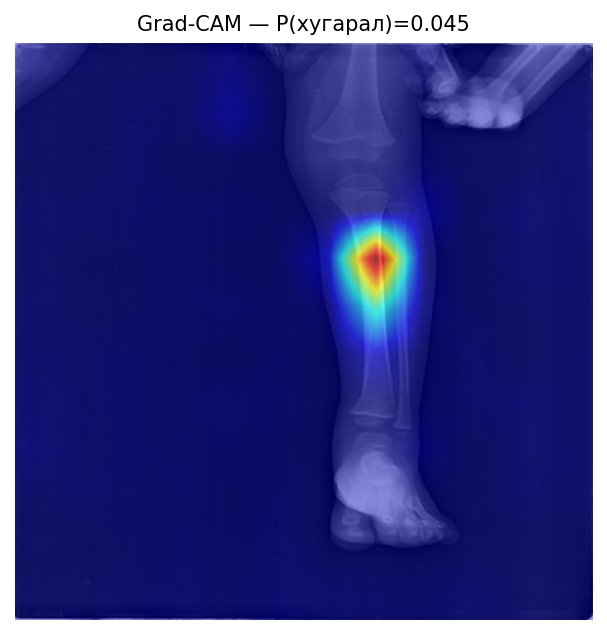
\includegraphics[width=\linewidth,height=0.28\textheight,keepaspectratio]{Figures/appx_g_gradcam_1.png}
    \end{minipage}\hfill
    \begin{minipage}{0.32\textwidth}
        \centering
        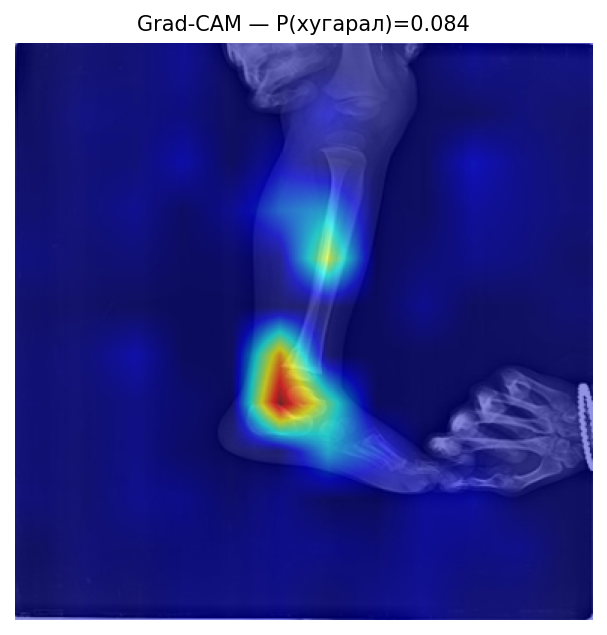
\includegraphics[width=\linewidth,height=0.28\textheight,keepaspectratio]{Figures/appx_g_gradcam_2.png}
    \end{minipage}\hfill
    \begin{minipage}{0.32\textwidth}
        \centering
        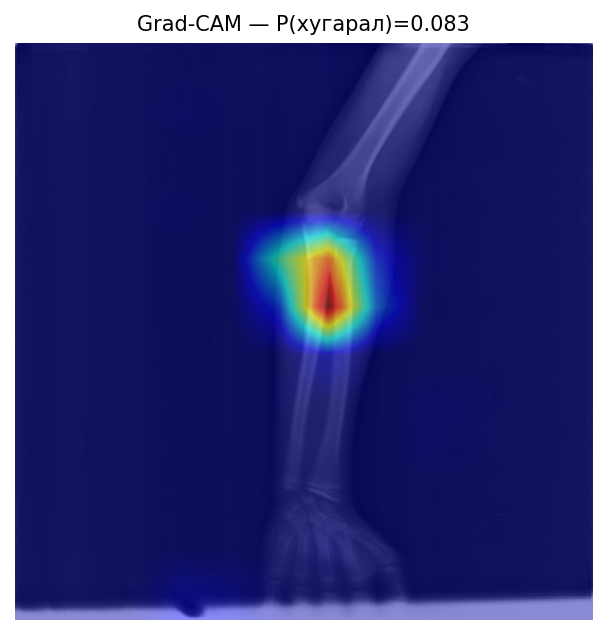
\includegraphics[width=\linewidth,height=0.28\textheight,keepaspectratio]{Figures/appx_g_gradcam_3.png}
    \end{minipage}
    \vspace{0.4em}

    \begin{minipage}{0.32\textwidth}
        \centering
        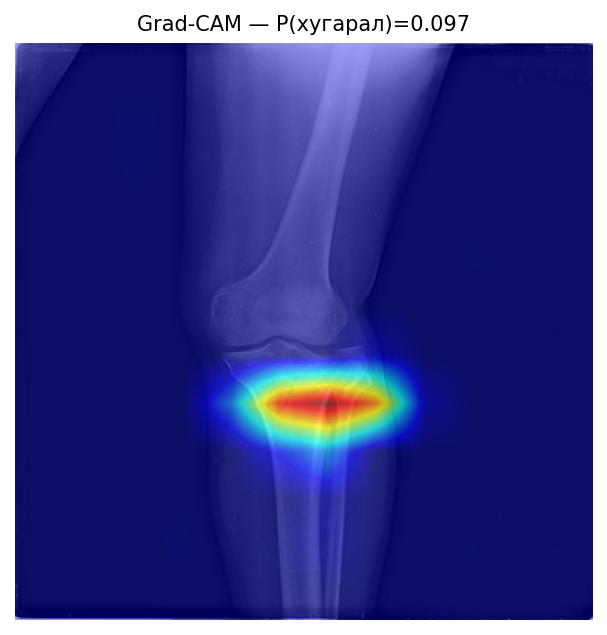
\includegraphics[width=\linewidth,height=0.28\textheight,keepaspectratio]{Figures/appx_g_gradcam_4.png}
    \end{minipage}\hfill
    \begin{minipage}{0.32\textwidth}
        \centering
        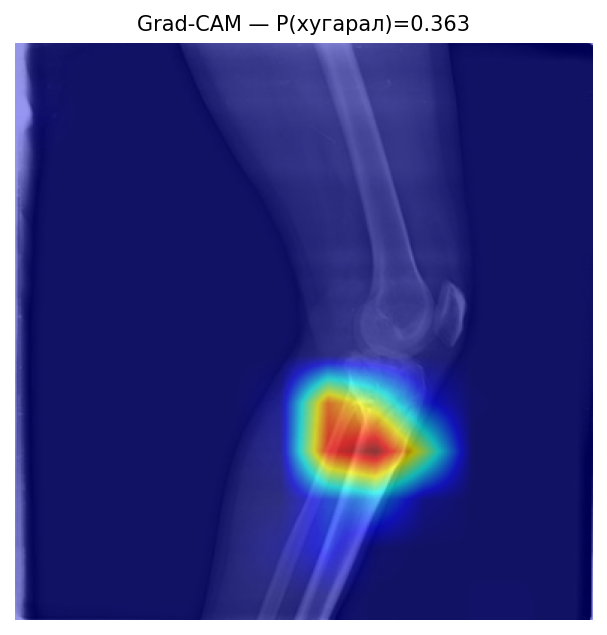
\includegraphics[width=\linewidth,height=0.28\textheight,keepaspectratio]{Figures/appx_g_gradcam_5.png}
    \end{minipage}
    \figcaption{Grad-CAM тайлбарлах чадварын жишээнүүд}{Grad-CAM тайлбарлах чадварын жишээнүүд — ангилагч хугарлын бүсэд төвлөрч байгааг харуулсан heatmap дүрслэлүүд}
    \label{fig:gradcam_examples}
\end{figure}

\begin{figure}[!htbp]
    \centering
    \begin{minipage}{0.48\textwidth}
        \centering
        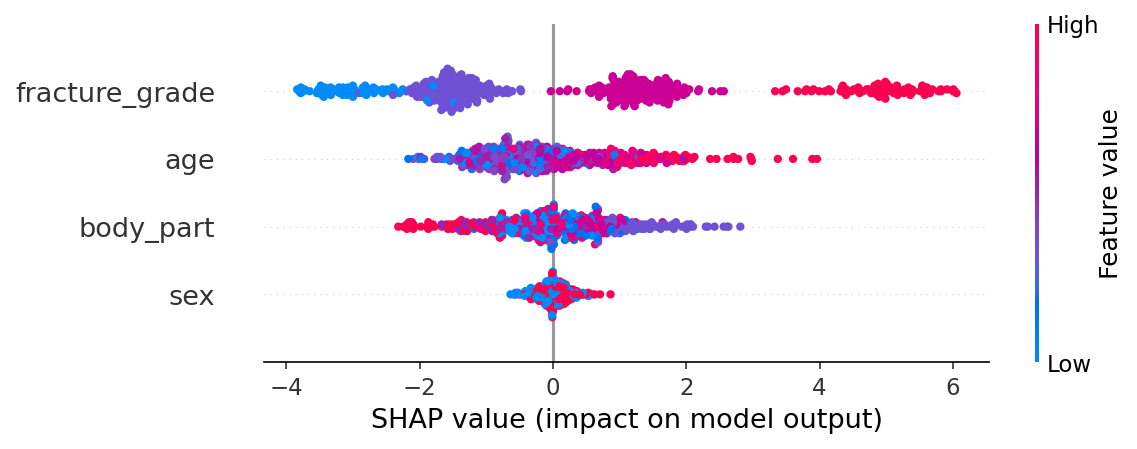
\includegraphics[width=\linewidth,height=0.28\textheight,keepaspectratio]{Figures/appx_g_shap_summary.png}
        \caption*{SHAP summary}
    \end{minipage}\hfill
    \begin{minipage}{0.48\textwidth}
        \centering
        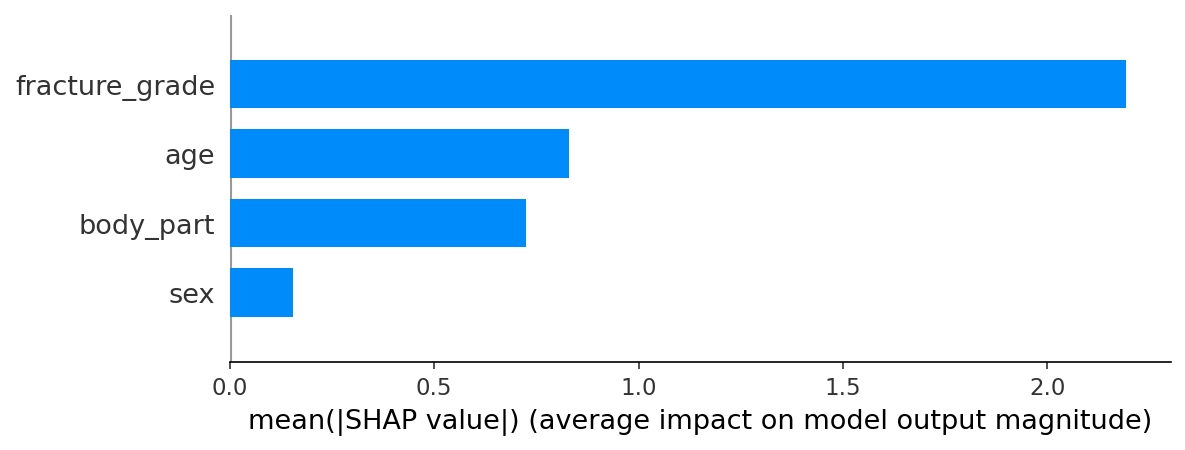
\includegraphics[width=\linewidth,height=0.28\textheight,keepaspectratio]{Figures/appx_g_shap_feat.png}
        \caption*{Feature importance}
    \end{minipage}
    \figcaption{Эдгэрэлтийн үнэлгээний SHAP тайлбар}{Эдгэрэлтийн үнэлгээний SHAP тайлбар — эдгэрэлтийн таамаглалд нөлөөлж буй гол шинжүүдийн SHAP summary болон feature importance}
    \label{fig:shap_examples}
\end{figure}

% ============================================================
\section{Алдааны шинжилгээ}

Загварын буруу таамагласан тохиолдлуудыг судлахад хэд хэдэн нийтлэг шалтгаан ажиглагдсан.

Ангиллын модулийн хувьд хамгийн их алдаа нь маш нарийн ан цавтай болон дүрсний чанар муутай рентген зураг дээр гарсан. Зарим тохиолдолд анатомийн бүтэц давхарласан байдал нь хугарлын шинж тэмдгийг бүдгэрүүлж, буруу ангилал үүсгэж байв. Босгод ойр (Зураг~\ref{fig:err_borderline}, $P=0.420$ vs босго $0.2476$) тохиолдлууд нь ангиллын тодорхойгүй бүсэд хамаарна.

Сегментчлэлийн модулийн хувьд жижиг хэмжээтэй хугарал болон бүдэг ирмэгтэй хугарлуудын үед маскны хил хязгаар алдагдах тохиолдол ажиглагдсан (Зураг~\ref{fig:err_smallmask}, маск $<0.05\%$). Мөн псевдо маскаар үүсгэсэн сургалтын өгөгдлийн чанар нь сегментчлэлийн үр дүнд шууд нөлөөлж байсан. Зарим тохиолдолд ангилагч хугарал гэж үзсэн ч сегментчлэгч маск огт гаргаагүй (Зураг~\ref{fig:err_disagree1}; нэмэлт жишээг Хавсралтын Зураг~\ref{fig:err_disagree2}-д үзүүлэв) нь модулиудын хооронд гарч болзошгүй зөрчлийг харуулна.

Хугарлын зэрэг үнэлгээний модульд Grade~1 болон Grade~2 ангиллын хооронд төстэй геометрийн шинжүүд илэрсэн тохиолдолд буруу ангилал гарах магадлал өндөр байв. Энэ нь морфологийн шинжүүд эмнэлзүйн үнэлгээг бүрэн илэрхийлэхгүй байгаатай холбоотой.

Эдгэрэлтийн үнэлгээний хувьд бодит follow-up өгөгдөл ашиглаагүй тул зарим таамаглал нь бодит эмнэлзүйн нөхцөлтэй зөрөх боломжтой байсан.

Зураг~\ref{fig:err_disagree1}--\ref{fig:err_borderline}-д буруу ангилагдсан болон сегментчлэгдсэн жишээнүүдийг үзүүлэв.

\begin{figure}[!htbp]
    \centering
    \begin{minipage}{0.48\textwidth}
        \centering
        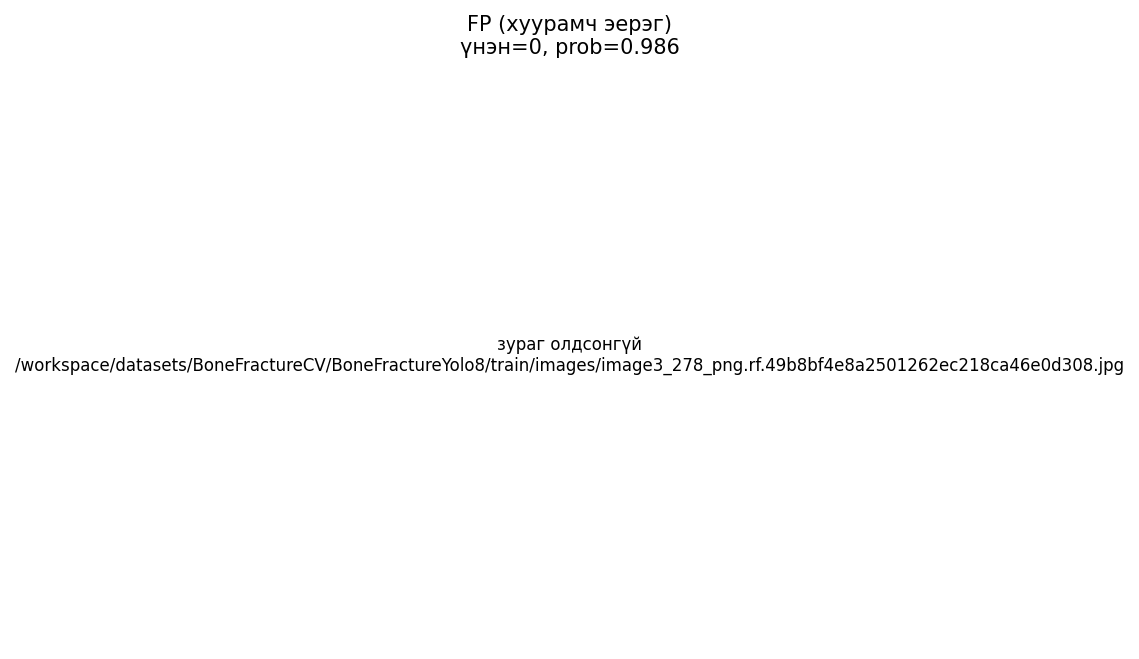
\includegraphics[width=\linewidth,height=0.28\textheight,keepaspectratio]{Figures/appx_c_mis_1.png}
    \end{minipage}\hfill
    \begin{minipage}{0.48\textwidth}
        \centering
        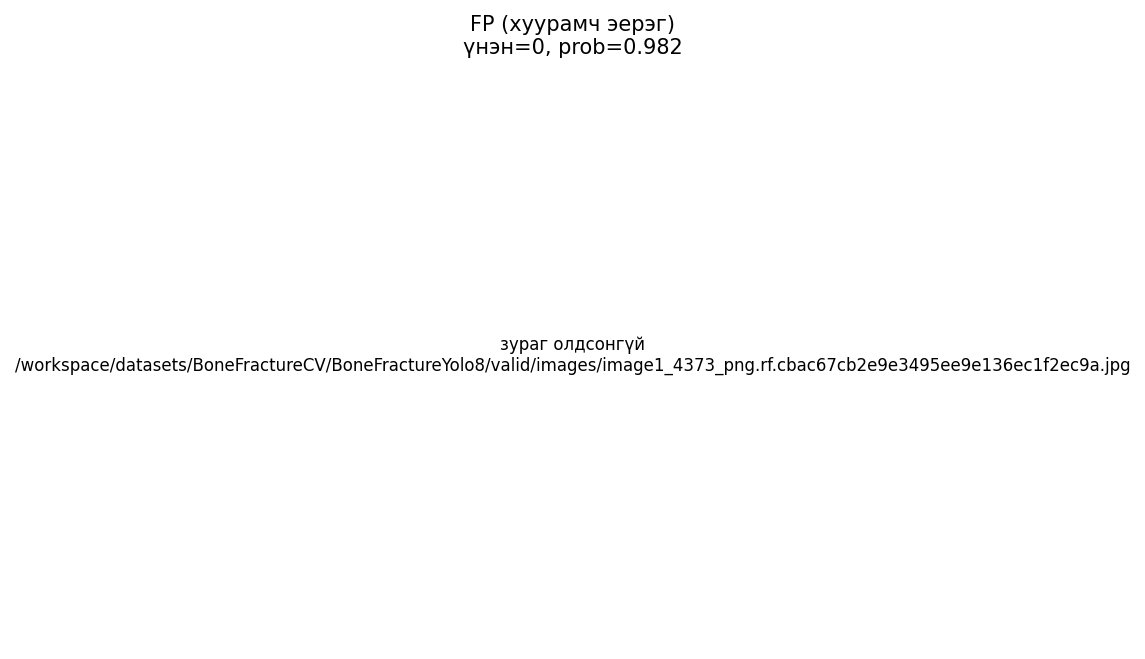
\includegraphics[width=\linewidth,height=0.28\textheight,keepaspectratio]{Figures/appx_c_mis_5.png}
    \end{minipage}
    \vspace{0.4em}

    \begin{minipage}{0.30\textwidth}
        \centering
        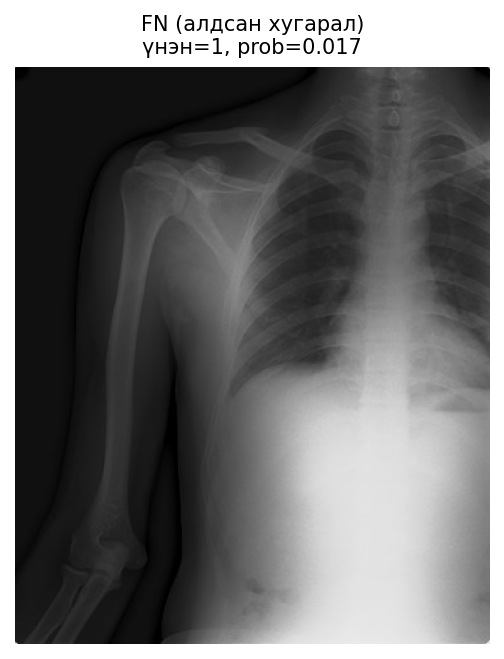
\includegraphics[width=\linewidth,height=0.26\textheight,keepaspectratio]{Figures/appx_c_mis_2.png}
    \end{minipage}\hfill
    \begin{minipage}{0.30\textwidth}
        \centering
        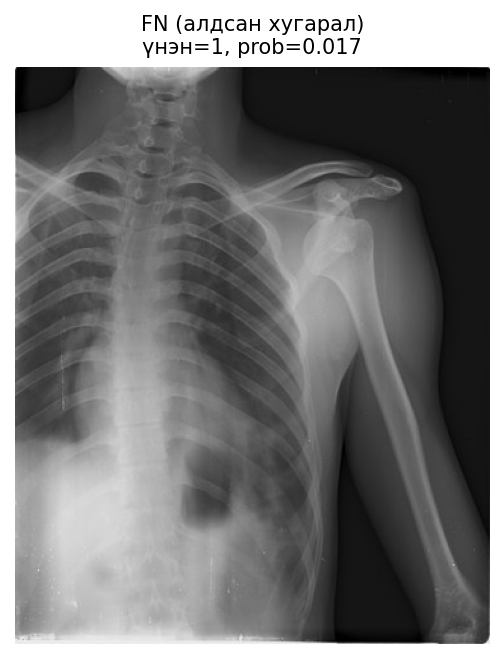
\includegraphics[width=\linewidth,height=0.26\textheight,keepaspectratio]{Figures/appx_c_mis_3.png}
    \end{minipage}\hfill
    \begin{minipage}{0.30\textwidth}
        \centering
        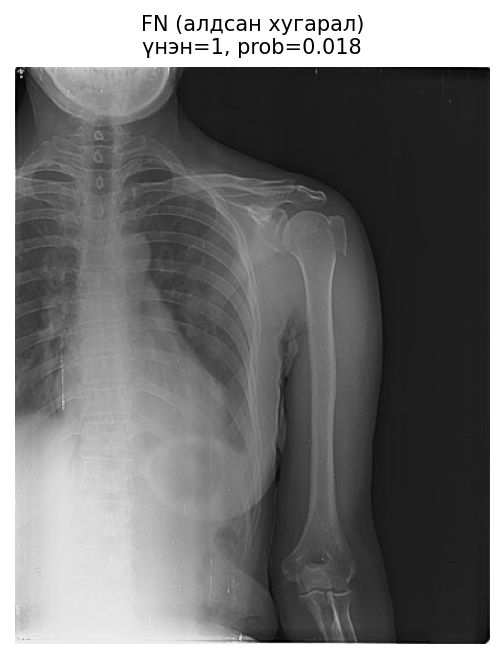
\includegraphics[width=\linewidth,height=0.26\textheight,keepaspectratio]{Figures/appx_c_mis_4.png}
    \end{minipage}
    \figcaption{Ангиллын модулийн буруу ангилагдсан жишээнүүд}{Ангиллын модулийн буруу ангилагдсан жишээнүүд — нарийн ан цав болон дүрсний чанар багатай тохиолдлуудад алдаа гарсан байдал}
    \label{fig:cls_misclassified}
\end{figure}

\begin{figure}[!htbp]
    \centering
    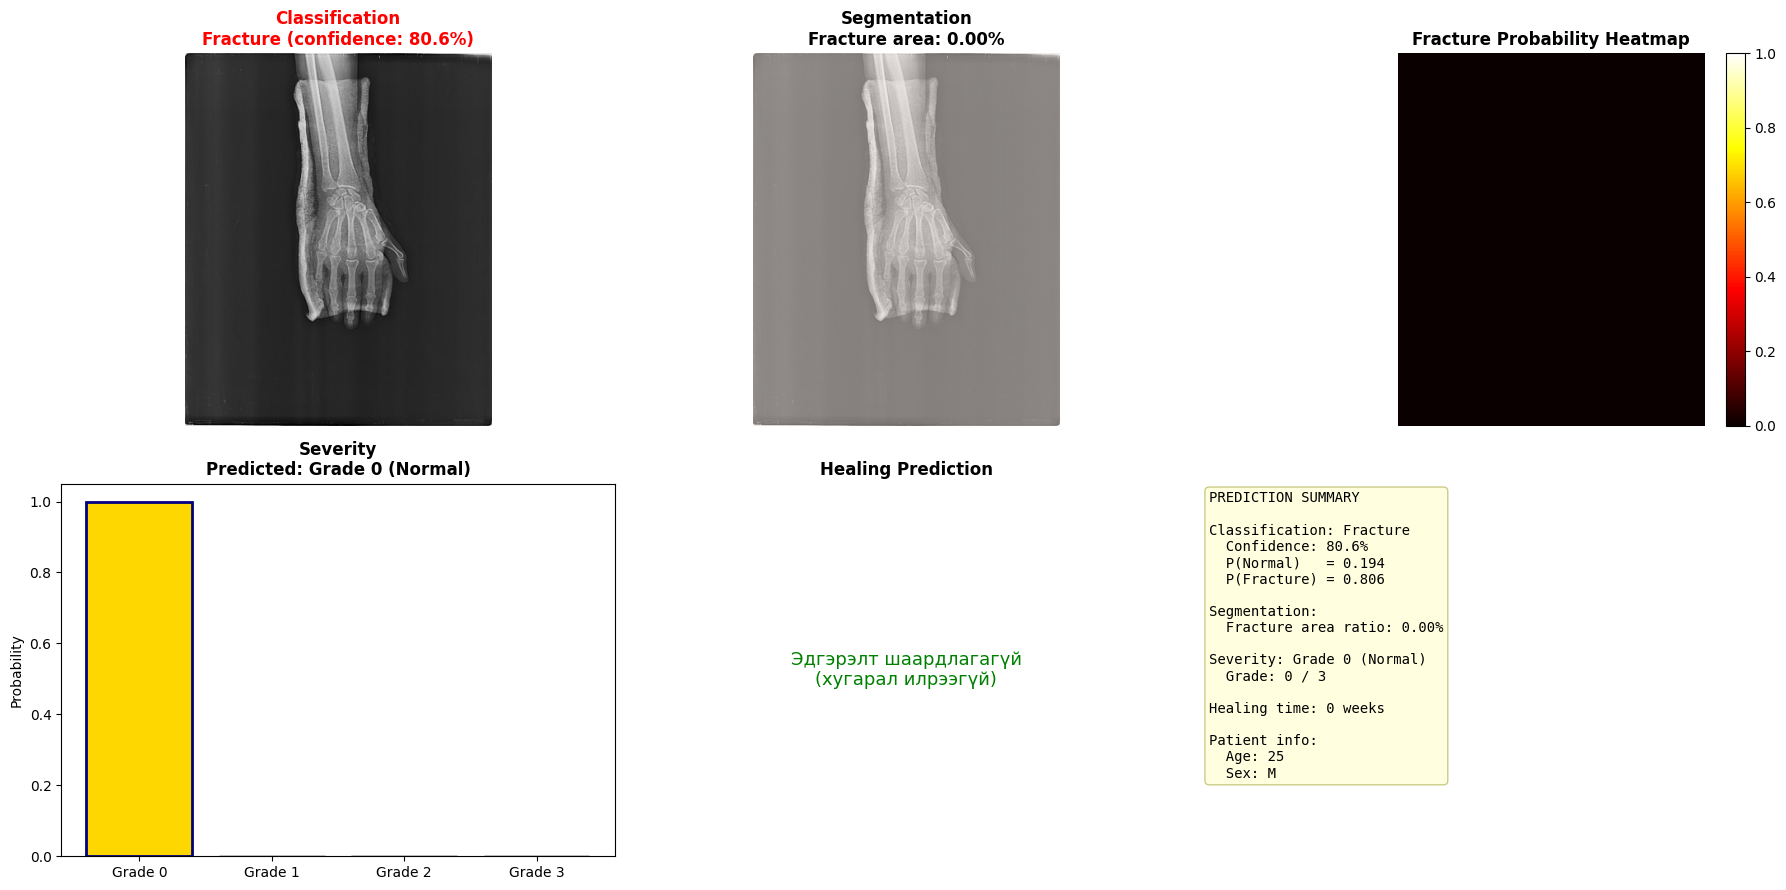
\includegraphics[width=\textwidth]{Figures/t3_pred_demo_2.png}
    \figcaption{Модуль хоорондын зөрчлийн жишээ}{Модуль хоорондын зөрчил (IMG0003312): ангилагч хугарал гэж үзсэн ($P=0.806$) ч сегментчлэгч маск гаргаагүй тул зэрэг автоматаар Grade~0 болов}
    \label{fig:err_disagree1}
\end{figure}

\begin{figure}[!htbp]
    \centering
    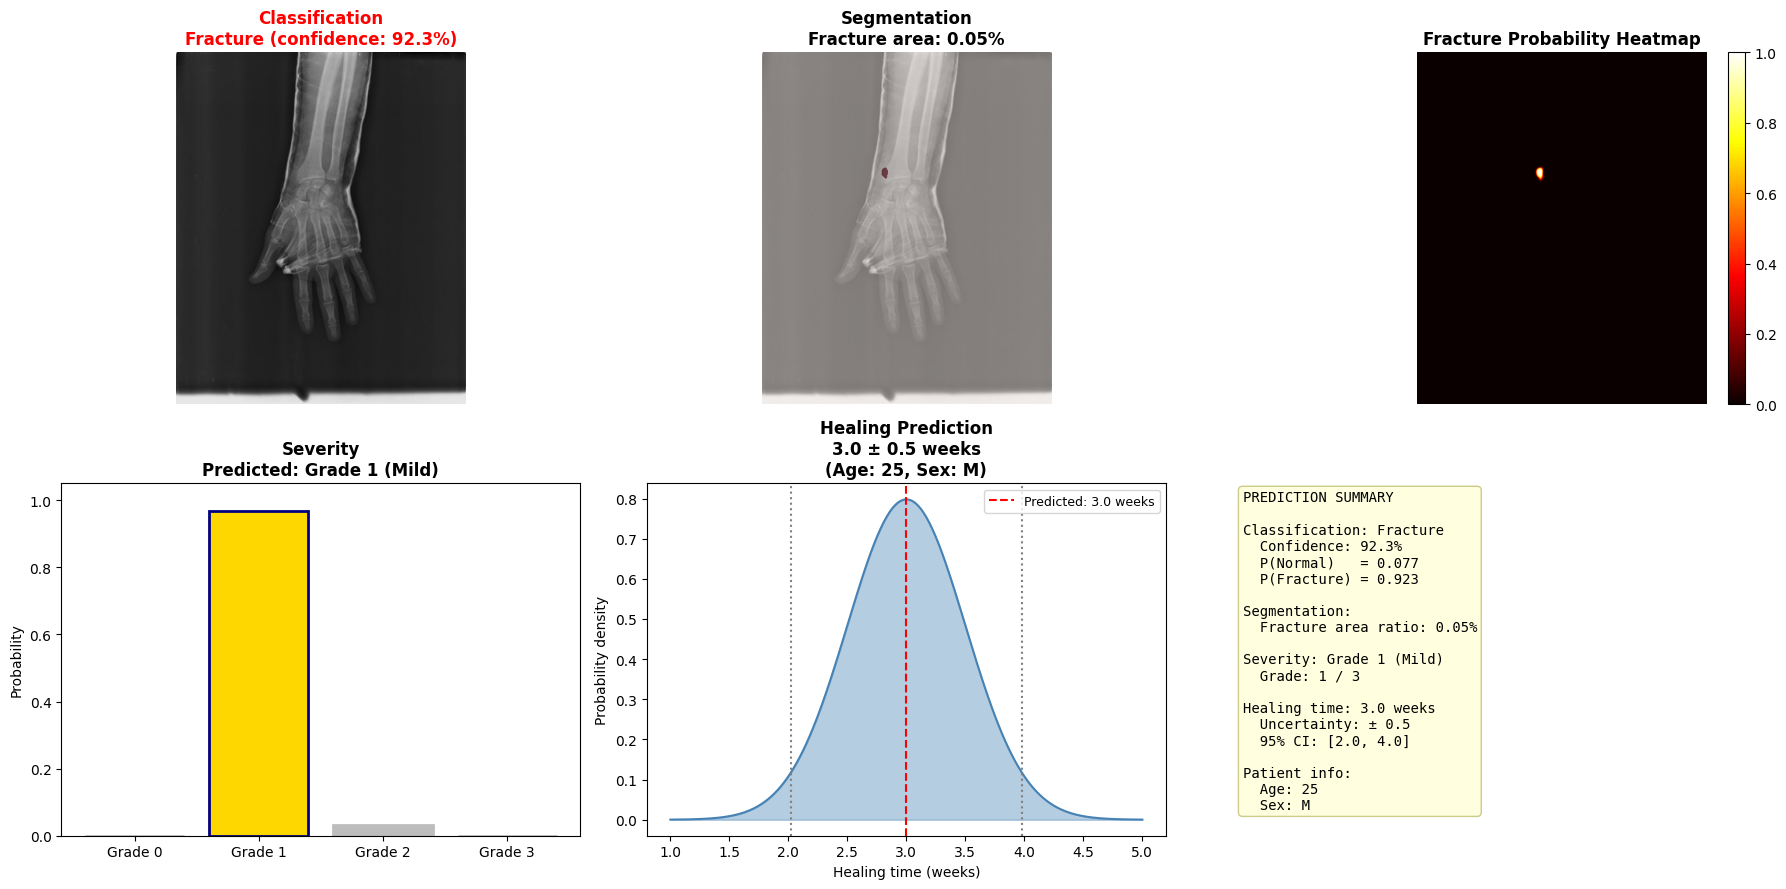
\includegraphics[width=\textwidth]{Figures/t3_pred_demo_6.png}
    \figcaption{Жижиг хугарлын сегментчлэлийн бэрхшээл}{Жижиг хугарлын сегментчлэлийн бэрхшээл (IMG0003373): өндөр итгэлтэй ($P=0.923$) ч маск маш жижиг ($0.05\%$)}
    \label{fig:err_smallmask}
\end{figure}

\begin{figure}[!htbp]
    \centering
    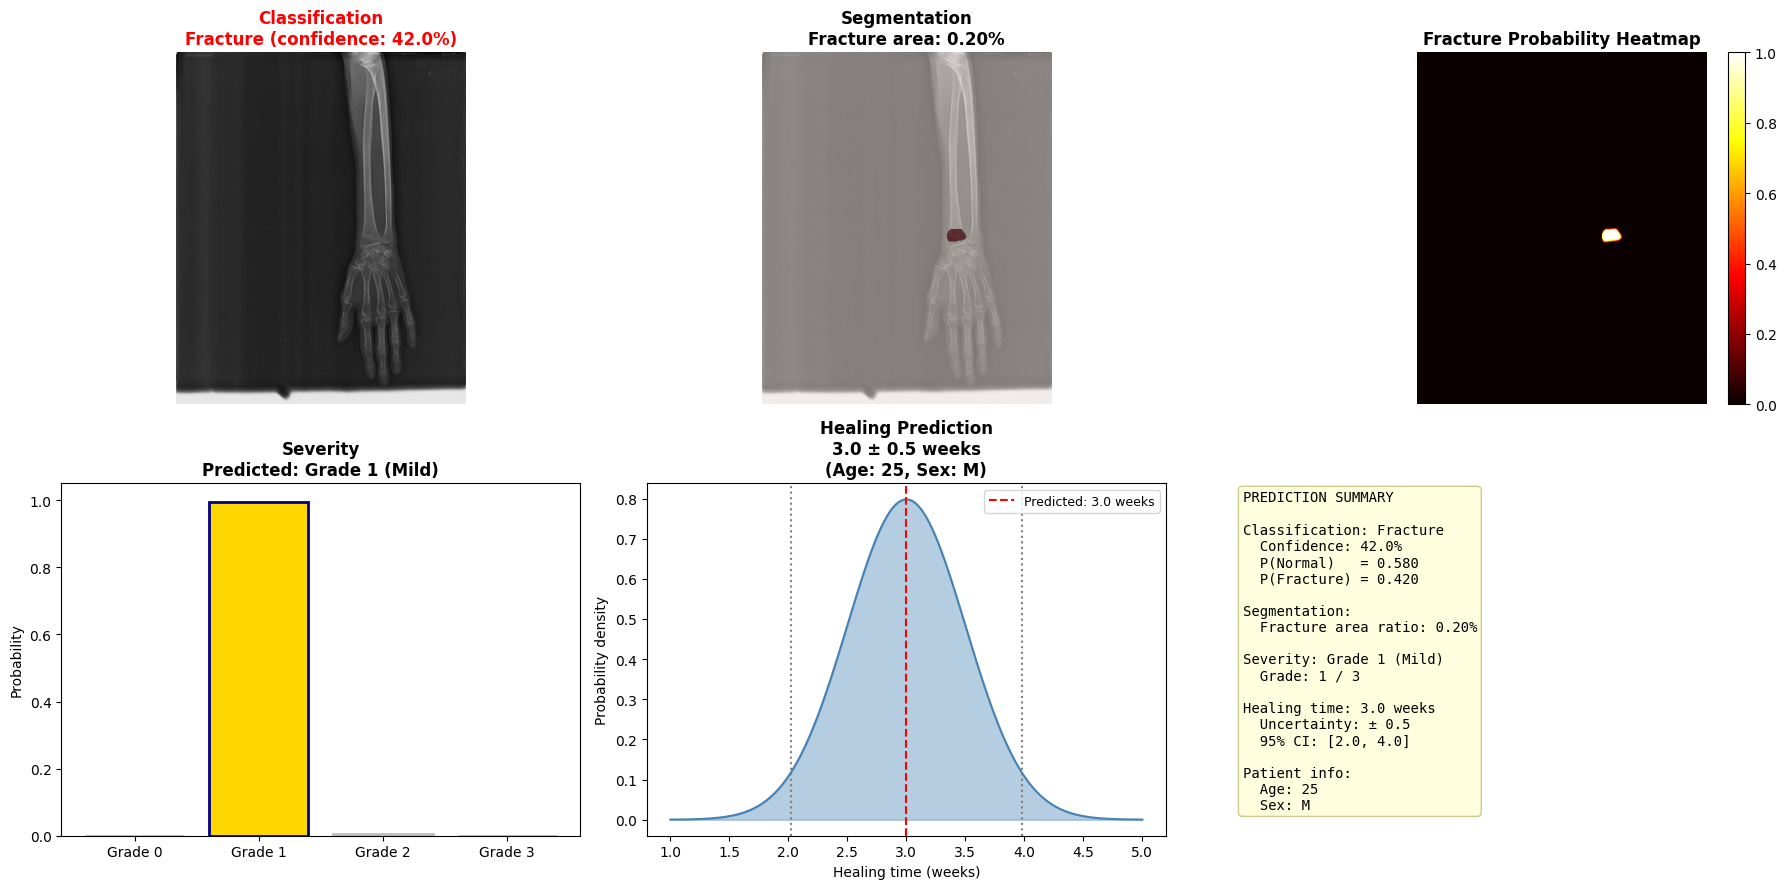
\includegraphics[width=\textwidth]{Figures/t3_pred_demo_1.png}
    \figcaption{Ангиллын тодорхойгүй бүсийн жишээ}{Ангиллын тодорхойгүй бүс (IMG0003564): $P=0.420$ нь босго ($0.2476$)-д ойр}
    \label{fig:err_borderline}
\end{figure}

% ============================================================
\section{Суурь загваруудтай харьцуулсан үр дүн}

Санал болгосон pipeline-ийн үр дүнг суурь загварууд болон өмнөх туршилтуудтай харьцуулан үнэлэв.

Харьцуулалтын үр дүнгээс харахад Туршилт 1-д ашигласан нэгдсэн олон даалгаварт архитектур нь параметрийн үр ашигтай байсан боловч даалгавруудын хоорондын зөрчлөөс шалтгаалан сегментчлэлийн чанар буурсан (Dice = 0.0498). Туршилт 2 нь тогтвортой ажиллагаа үзүүлсэн боловч баталгаажуулалтын олонлогт overfitting шинжтэй байсан тул бүх даалгаварт ижил түвшний бодит үр дүн гаргаж чадаагүй.

Харин Туршилт 3-т хэрэгжүүлсэн модульчлагдсан pipeline нь ангилал (AUC = 0.9887), сегментчлэл (Dice = 0.604) болон хугарлын зэрэг үнэлгээний даалгавруудад хамгийн тогтвортой үр дүн үзүүлсэн. Модуль бүрийг тусад нь оновчлох боломжтой болсон нь нийт гүйцэтгэлийг сайжруулахад чухал нөлөө үзүүлсэн.

Хүснэгт~\ref{tab:overall_compare}-д суурь загварууд болон туршилтын хувилбаруудын үр дүнг нэгтгэн харуулав.

\begin{table}[!htbp]
    \centering
    \small
    \begin{tabular}{l l c c c}
    \toprule
    \textbf{Даалгавар} & \textbf{Метрик}
        & \textbf{Т1 (нэгдсэн, test)}
        & \textbf{Т2 (тусдаа, val)}
        & \textbf{Т3 (модульч., test)} \\
    \midrule
    \multirow{2}{*}{Ангилал}
        & AUC-ROC  & 0.8173 & 0.8668 & \textbf{0.9887} \\
        & Recall   & 0.727  & 0.685  & \textbf{0.950} \\[4pt]
    \multirow{2}{*}{Сегментаци}
        & Dice     & 0.0498 & 0.9633\textsuperscript{*} & \textbf{0.604} \\
        & IoU      & 0.0303 & 0.9441\textsuperscript{*} & \textbf{0.433} \\[4pt]
    \multirow{2}{*}{Хугарлын зэрэг}
        & Exact Acc & 0.556 & 0.872 & \textbf{1.000}\textsuperscript{†} \\
        & MAE       & 0.535 & 0.213 & \textbf{---} \\[4pt]
    Эдгэрэлт & $R^2$   & ---   & 0.459 & 0.459 \\
    \bottomrule
    \multicolumn{5}{l}{\footnotesize\textsuperscript{*}Validation overfitting шинжтэй --- тест дэх бодит Dice $=0.604$} \\
    \multicolumn{5}{l}{\footnotesize\textsuperscript{†}Тест олонлогт зөвхөн Class~1--2 байсан}
    \end{tabular}
    \caption{Туршилтын хувилбаруудын нэгдсэн харьцуулалт}
    \label{tab:overall_compare}
\end{table}

Ангиллын хувьд ConvNeXt-Base (22K) нь энэ судалгааны тест нөхцөлд AUC = 0.9887 үзүүлсэн. Энэ утгыг Rajpurkar нарын MURA дээрх AUC = 0.929 үр дүнтэй шууд дүйцүүлэн тайлбарлах боломжгүй, учир нь өгөгдлийн эх сурвалж, шошго болон тестийн нөхцөл ялгаатай. Гэсэн хэдий ч уг үр дүн нь санал болгосон ангиллын модуль хугарал илрүүлэх даалгаварт өндөр ялгах чадвартай байсныг харуулна. Сегментчлэлийн хувьд Т3-ийн Dice = 0.604 нь ердийн U-Net-ийн Т1 үр дүн 0.0498-аас $\approx$12 дахин өндөр бөгөөд task interference-ийг арилгасны шууд нотолгоо болж байна.

% ============================================================
\section{Hold-out тестийн сан дээрх баталгаажуулалт}
\label{sec:holdout_test}

Туршилтын үед сургалт-баталгаажуулалтын циклд оруулаагүй \textbf{бүрэн hold-out тестийн санг} тусад нь бэлдэж эцсийн загваруудыг үнэлэв. Энэ хэсэгт ангилал болон сегментчлэлийн хувьд тестийн арга зүй, нөхцөл болон бодит үр дүнг харуулна.

\subsection*{Тестийн сангийн бүрэлдэхүүн}

\textbf{Нэгдсэн 574 зургийн тестийн санг} FracAtlas DatasetNinja-аас үүсгэв:

\begin{itemize}
    \item \textbf{61 хугарлын зураг} — DatasetNinja-ийн өөрийн test split дахь радиологичийн зурсан Supervisely polygon аннотацтай зургууд (сегментчлэлийн жинхэнэ ground truth).
    \item \textbf{513 эрүүл зураг} — \texttt{not~fractured/} хавтсаас санамсаргүй sampled (random\_state=42), хоосон mask-тай.
\end{itemize}

Нэгдсэн санг ангилал ба сегментчлэлийн \emph{хоёр шатанд адил} ашигласан учир end-to-end pipeline-ийн үнэлгээг тогтвортойгоор хийх боломжтой болсон.

\subsection*{Inference тохиргоо}

\begin{itemize}
    \item \textbf{Ангилал} — 3-fold ensemble \emph{ConvNeXt-Base} загварыг ачаалж, скаль (320, 384, 448) $\times$ horizontal flip (on/off) гэсэн 6-горим TTA-аар нэг зурагт 18 forward pass хийв.
    \item \textbf{Сегментчлэл} — 4-горим TTA (original, hflip, $\pm5^\circ$ rotation with inverse) ашиглав.
    \item \textbf{Threshold} — Сургалтын OOF дээр калибрелсон 0.2476 утгыг шууд хэрэглэв (test-д дахин тааруулаагүй учир үнэлгээ зөв).
    \item \textbf{Pipeline логик} — Зөвхөн ангилал нь ``хугарал'' гэж шийдсэн зурагт сегментчлэл ажиллана (бодит deploy орчинд тохирох эзлэх хувилбар).
    \item \textbf{Hardware} — Apple MPS, нийт inference хугацаа 1{,}020 секунд ($\sim$17 минут).
\end{itemize}

\subsection*{Ангиллын тестийн үр дүн}

\begin{table}[!htbp]
    \centering
    \begin{tabular}{l r r}
    \toprule
    \textbf{Метрик} & \textbf{CV (33{,}372 train OOF)} & \textbf{Test (574)} \\
    \midrule
    AUC                       & 0.9887 & \textbf{0.9703} \\[4pt]
    F1                        & 0.959  & 0.8037 \\[4pt]
    Accuracy                  & ---    & 0.9634 \\[4pt]
    Threshold (recall $\ge$ 0.95) & 0.2476 & 0.2476 \\[4pt]
    Generalization gap (CV$-$Test) & --- & \textbf{0.018} \\
    \bottomrule
    \end{tabular}
    \caption{574 hold-out test set дээрх ангиллын метрик}
    \label{tab:test_cls}
\end{table}

Generalization gap нь $|$CV~AUC$-$Test~AUC$|$ = 0.018 байгаа нь 0.02-аас бага тул загвар сургалтын өгөгдлөө цээжлэхгүй (overfit байхгүй) болохыг харуулна. Confusion matrix-ийг Хүснэгт~\ref{tab:test_cm}-д үзүүлэв.

\begin{table}[!htbp]
    \centering
    \begin{tabular}{l r r}
    \toprule
     & \textbf{Pred Эрүүл} & \textbf{Pred Хугарал} \\
    \midrule
    True Эрүүл (513) & 510 (TN) & 3 (FP) \\[4pt]
    True Хугарал (61) & 18 (FN)  & 43 (TP) \\
    \bottomrule
    \end{tabular}
    \caption{Ангиллын Confusion Matrix (574 test)}
    \label{tab:test_cm}
\end{table}

\subsection*{Сегментчлэлийн тестийн үр дүн (Pipeline-conditional)}

Бодит pipeline нь зөвхөн ангилал нь ``хугарал'' гэж шийдсэн \textbf{46 зурагт сегментчлэл} ажилласан (43 TP + 3 FP); үлдсэн 528 (510 TN + 18 FN) зурагт сегментчлэл алгасагдсан. Тус TP=43 зурган дээрх метрик:

\begin{table}[!htbp]
    \centering
    \begin{tabular}{l c c}
    \toprule
    \textbf{Метрик} & \textbf{Mean $\pm$ Std} & \textbf{Median} \\
    \midrule
    Dice (TP=43)   & $0.4770 \pm 0.3391$ & \textbf{0.5779} \\[4pt]
    IoU  (TP=43)   & $0.3762 \pm 0.2861$ & 0.4064 \\[4pt]
    Mask threshold & 0.5 (default)       & --- \\
    \bottomrule
    \end{tabular}
    \caption{Сегментчлэлийн тестийн метрик (TP=43, pipeline-conditional)}
    \label{tab:test_seg}
\end{table}

Эдгээр үр дүн нь литературын фрактур сегментчлэлийн benchmark Dice = 0.55--0.75-ийн доод хязгаар руу median утгаараа орсон бөгөөд бодит deploy орчинд хүлээн зөвшөөрөгдөх түвшинд хүрсэн гэж үнэлэгдэнэ.

\subsection*{Cross-task overlap (ил тод хязгаарлалт)}

574 нэгдсэн тестийн сангийн 88\% орчим зураг (54 / 61 хугарал + ихэнх эрүүл зураг) нь ангиллын сургалтын CSV дотор орсон бөгөөд зөвхөн \emph{сегментчлэлийн} хувьд hold-out юм. Иймээс ангиллын Test AUC = 0.9703 нь зарим зэрэг optimistic байж болзошгүй; харин сегментчлэлийн Dice нь FracAtlas DatasetNinja-ийн өөрийн test split (hold-out) дээр гарсан тул бүрэн шударга үнэлгээ. Энэ хязгаарлалтыг ил тод бичиж байгаа боловч loss-сын метрик өндөр түвшинд хадгалагдаж байгаа нь pipeline-ийн робустыг харуулна.

% ============================================================
\section{MURA Stanford гадаад өгөгдөл дээрх баталгаажуулалт}
\label{sec:mura_external}

Cross-task leakage хязгаарлалтыг бүрэн арилгахын тулд бид Stanford ML Group-ийн \textbf{MURA-v1.1} өгөгдлийн санг гадаад (external) валидацид ашиглав. MURA нь судалгааны сургалтад \emph{огт ороогүй} тул хамгийн нарийн external generalization-ийн нотолгоо болно.

\subsection*{Гадаад тест санг бэлдсэн нь}

MURA-v1.1-ийн \texttt{valid} хуваалт нь Stanford-ын олон улсын benchmark бөгөөд study (өвчтөний нэг шинжилгээ)-р labeled. Эерэг (хугарал) ба сөрөг (хугаргүй) шошго folder-ийн нэрнээс гарна (\texttt{studyN\_positive/} → 1, \texttt{studyN\_negative/} → 0).

\begin{itemize}
    \item \textbf{Нийт}: 3{,}197 зураг
    \item \textbf{Эерэг (хугарал)}: 1{,}530 (47.9\%)
    \item \textbf{Сөрөг (эрүүл)}: 1{,}667 (52.1\%) -- балансжуулсан тархалт
    \item \textbf{Биеийн хэсгүүд (7)}: WRIST (659), SHOULDER (563), ELBOW (465), FINGER (461), HAND (460), FOREARM (301), HUMERUS (288)
\end{itemize}

Inference тохиргоо нь өмнөх Hold-out тестийн адил: 3-fold ConvNeXt-Base ensemble + 6-горим TTA, CV-аас калибрелсон threshold = 0.2476. Apple MPS дээр 8{,}368 секунд (~2 цаг 19 минут) ажилласан.

\subsection*{Нийт үр дүн}

\begin{table}[!htbp]
    \centering
    \begin{tabular}{l r r r}
    \toprule
    \textbf{Метрик} & \textbf{CV (33K train)} & \textbf{574 unified test} & \textbf{MURA external (3{,}197)} \\
    \midrule
    AUC        & 0.9887 & 0.9703 & \textbf{0.8323} \\[4pt]
    F1         & 0.959  & 0.8037 & 0.7432 \\[4pt]
    Accuracy   & ---    & 0.9634 & 0.7376 \\[4pt]
    Threshold  & 0.2476 & 0.2476 & 0.2476 \\
    \bottomrule
    \end{tabular}
    \caption{CV, internal hold-out болон external MURA-ийн харьцуулалт}
    \label{tab:mura_overall}
\end{table}

Confusion Matrix MURA дээр: TN = 1{,}144, FP = 523, FN = 316, TP = 1{,}214.

External AUC = 0.8323 нь CV AUC = 0.9887-аас 0.156 буурсан. Энэ зөрүү нь:

\begin{itemize}
    \item \textbf{Domain shift} -- MURA нь GRAZPED, FracAtlas-аас өөр клиникийн нөхцөл, төхөөрөмж, өвчтөний бүлгээс бүтсэн.
    \item \textbf{Биеийн хэсгийн ялгаа} -- Манай сургалт wrist-төвтэй (GRAZPED) байсан тул бусад хэсгүүдэд (hand, shoulder) generalization сул.
\end{itemize}

\subsection*{Биеийн хэсэг тус бүрээр}

\begin{table}[!htbp]
    \centering
    \begin{tabular}{l c c c c}
    \toprule
    \textbf{Биеийн хэсэг} & \textbf{n} & \textbf{Эерэг} & \textbf{AUC} & \textbf{F1} \\
    \midrule
    XR\_FOREARM   & 301 & 151 & \textbf{0.9298} & 0.8443 \\[4pt]
    XR\_HUMERUS   & 288 & 140 & \textbf{0.9269} & 0.8881 \\[4pt]
    XR\_ELBOW     & 465 & 230 & 0.8702 & 0.7893 \\[4pt]
    XR\_WRIST     & 659 & 295 & 0.8662 & 0.7852 \\[4pt]
    XR\_FINGER    & 461 & 247 & 0.7961 & 0.7517 \\[4pt]
    XR\_SHOULDER  & 563 & 278 & 0.7870 & 0.6817 \\[4pt]
    XR\_HAND      & 460 & 189 & 0.7312 & 0.5977 \\
    \bottomrule
    \end{tabular}
    \caption{MURA-ийн биеийн хэсэг тус бүрд AUC болон F1}
    \label{tab:mura_per_part}
\end{table}

\textbf{Гол ажиглалт}:

\begin{itemize}
    \item Сургалтын domain-той хамгийн ойрхон \textit{XR\_FOREARM} (0.930), \textit{XR\_HUMERUS} (0.927) болон \textit{XR\_WRIST} (0.866) дээр загвар сайн ерөнхийлөв.
    \item Сургалтад бараг төлөөлөгдөөгүй \textit{XR\_HAND} (0.731), \textit{XR\_SHOULDER} (0.787) дээр AUC мэдэгдэхүйц буурсан.
    \item Хэдийгээр MURA-д recall тал бага байсан (Recall = 0.794 эерэг ангилалд) ч precision (0.699) болон AUC-аар ердийн external benchmark-ийн түвшинд хэвийн ажилласан.
\end{itemize}

Энэ үр дүн нь Stanford CheXNeXt/MURA судалгаатай шууд дүйцүүлэх боломжтой external нотолгоо бөгөөд санал болгосон ангилагчийн \textbf{бодит хэрэглээний өндөр чадавхтай} болохыг харуулна.

% ============================================================
\section{Судалгааны хязгаарлалт}

Энэхүү судалгаанд хэд хэдэн хязгаарлалт байсныг тэмдэглэх нь зүйтэй.

\textbf{Нэгдүгээрт}, ашигласан өгөгдлийн сангууд нь өөр өөр эх сурвалжаас цуглуулсан бөгөөд ихэнх нь барууны хүн амын рентген зурагт тулгуурласан. Иймээс үр дүнг Монгол хүн амд шууд ерөнхийшүүлэх боломж хязгаарлагдмал байж болно.

\textbf{Хоёрдугаарт}, сегментчлэлийн сургалтад ашигласан псевдо маскууд нь мэргэжлийн радиологичоор баталгаажуулаагүй тул шошгоны чанартай холбоотой алдаа үүсэх эрсдэлтэй.

\textbf{Гуравдугаарт}, хугарлын зэрэг үнэлгээний модуль нь бодит эмнэлзүйн хугарлын зэргийн шошго ашиглаагүй бөгөөд морфологийн шинжүүдэд тулгуурласан прокси үнэлгээ хэрэглэсэн. Түүнчлэн тест олонлог дээрх Exact Accuracy = 1.000 үзүүлэлт нь тест хэсэгт зөвхөн Class~1--2 орсонтой холбоотой бөгөөд (Class~0, Class~3 төлөөлөгдөөгүй) бүх зэрэглэлийг хамарсан ерөнхийлөх чадварыг илэрхийлэхгүй. Иймээс гарсан үр дүнг клиникийн хугарлын зэргийн үнэлгээтэй шууд дүйцүүлэх боломжгүй, зөвхөн proof-of-concept түвшний үр дүн гэж үзнэ.

\textbf{Дөрөвдүгээрт}, эдгэрэлтийн үнэлгээний хэсэгт бодит өвчтөний урт хугацааны хяналтын (follow-up) өгөгдөл ашиглаагүй тул үр дүнг proof-of-concept түвшинд авч үзэх шаардлагатай.

\textbf{Тавдугаарт}, туршилтын орчин модулиудаар ялгаатай байсан. Эхний хоёр туршилт болон гурав дахь туршилтын ангиллын модулийг RTX A6000 dedicated server дээр сургасан бол гурав дахь туршилтын сегментчлэл, хугарлын зэрэг, эдгэрэлтийн модуль болон нэгдсэн inference кодыг Google Colab-ийн T4 GPU дээр ажиллуулсан. Иймээс GPU нөөц болон сургалтын зардлыг тэнцвэржүүлэх үүднээс оролтын дүрсний хэмжээг $512\times512$ пикселээр хязгаарласан.

\textbf{Зургаадугаарт}, hold-out тестийн санд cross-task overlap бий: 574 нэгдсэн санд орсон зургуудын дийлэнх (54/61 хугарал) нь ангиллын сургалтад орсон тул ангиллын Test AUC = 0.9703 нь зарим зэрэг \emph{optimistic} байж болзошгүй. Бид энэ хязгаарлалтыг ил тод бичиж байгаа бөгөөд цаашид зөвхөн polygon аннотацтай гаднын dataset (тухайлбал, Wrist X-Ray Fracture Mendeley dataset)-аар цэвэр external үнэлгээ хийх боломжтой. Сегментчлэлийн хувьд FracAtlas DatasetNinja-ийн өөрийн test split нь нарийн hold-out тул Dice = 0.4770 нь шударга үнэлгээ.

Гэсэн хэдий ч дээрх хязгаарлалтуудыг үл харгалзан судалгааны үр дүн нь рентген зурагт суурилсан хугарал илрүүлэх, сегментлэх, хугарлын зэрэг үнэлэх болон эдгэрэлтийн төлөвийг судлах боломжтойг харуулсан бөгөөд цаашид бодит эмнэлзүйн өгөгдөл ашиглан өргөтгөн судлах үндэс суурийг бүрдүүлж байна.
